% This is the Reed College LaTeX thesis template. Most of the work
% for the document class was done by Sam Noble (SN), as well as this
% template. Later comments etc. by Ben Salzberg (BTS). Additional
% restructuring and APA support by Jess Youngberg (JY).
% Your comments and suggestions are more than welcome; please email
% them to cus@reed.edu
%
% See http://web.reed.edu/cis/help/latex.html for help. There are a
% great bunch of help pages there, with notes on
% getting started, bibtex, etc. Go there and read it if you're not
% already familiar with LaTeX.
%
% Any line that starts with a percent symbol is a comment.
% They won't show up in the document, and are useful for notes
% to yourself and explaining commands.
% Commenting also removes a line from the document;
% very handy for troubleshooting problems. -BTS

% As far as I know, this follows the requirements laid out in
% the 2002-2003 Senior Handbook. Ask a librarian to check the
% document before binding. -SN

%%
%% Preamble
%%
% \documentclass{<something>} must begin each LaTeX document
\documentclass[12pt,twoside]{reedthesis}
% Packages are extensions to the basic LaTeX functions. Whatever you
% want to typeset, there is probably a package out there for it.
% Chemistry (chemtex), screenplays, you name it.
% Check out CTAN to see: http://www.ctan.org/
%%
\usepackage{graphicx,latexsym}
\usepackage{amssymb,amsthm,amsmath}
\usepackage{longtable,booktabs,setspace}
\usepackage{chemarr} %% Useful for one reaction arrow, useless if you're not a chem major
\usepackage[hyphens]{url}
\usepackage{rotating}
\usepackage{natbib}
\usepackage{listings}
\usepackage{tikz}
\usepackage{xcolor,colortbl}
\usepackage{float}
\usepackage{algorithm}
\usepackage[noend]{algpseudocode}



\newenvironment{codeexample}[1][htb]
{\floatname{algorithm}{Code Example}%\renewcommand{\algorithmcfname}{Code example}% Update algorithm name
	\begin{algorithm}[#1]%
	}{\end{algorithm}}


\lstset
{ %Formatting for code in appendix
	basicstyle=\footnotesize,
	numbers=left,
	stepnumber=1,
	showstringspaces=false,
	tabsize=4,
	breaklines=true,
	breakatwhitespace=false,
}

% Comment out the natbib line above and uncomment the following two lines to use the new
% biblatex-chicago style, for Chicago A. Also make some changes at the end where the
% bibliography is included.
%\usepackage{biblatex-chicago}
%\bibliography{thesis}

% \usepackage{times} % other fonts are available like times, bookman, charter, palatino

\newcommand{\ceil}[1]{\lceil #1 \rceil}
\newcommand{\floor}[1]{\lfloor #1 \rfloor}



\title{My Final College Paper}
\author{Your R. Name}
% The month and year that you submit your FINAL draft TO THE LIBRARY (May or December)
\date{May 200x}
\division{Mathematics and Natural Sciences}
\advisor{Advisor F. Name}
%If you have two advisors for some reason, you can use the following
%\altadvisor{Your Other Advisor}
%%% Remember to use the correct department!
\department{Mathematics}
% if you're writing a thesis in an interdisciplinary major,
% uncomment the line below and change the text as appropriate.
% check the Senior Handbook if unsure.
%\thedivisionof{The Established Interdisciplinary Committee for}
% if you want the approval page to say "Approved for the Committee",
% uncomment the next line
%\approvedforthe{Committee}

\setlength{\parskip}{0pt}
%%
%% End Preamble
%%
%% The fun begins:
\begin{document}

  \maketitle
  \frontmatter % this stuff will be roman-numbered
  \pagestyle{empty} % this removes page numbers from the frontmatter

% Acknowledgements (Acceptable American spelling) are optional
% So are Acknowledgments (proper English spelling)
    \chapter*{Acknowledgments}
	I want to thank a few people.

% The preface is optional
% To remove it, comment it out or delete it.
    \chapter*{Preface}
	This is an example of a thesis setup to use the reed thesis document class.



    \chapter*{List of Abbreviations}
		You can always change the way your abbreviations are formatted. Play around with it yourself, use tables, or come to CUS if you'd like to change the way it looks. You can also completely remove this chapter if you have no need for a list of abbreviations. Here is an example of what this could look like:

	\begin{table}[h]
	\centering % You could remove this to move table to the left
	\begin{tabular}{ll}
		\textbf{ABC}  	&  American Broadcasting Company \\
		\textbf{CBS}  	&  Columbia Broadcasting System\\
		\textbf{CDC}  	&  Center for Disease Control \\
		\textbf{CIA}  	&  Central Intelligence Agency\\
		\textbf{CLBR} 	&  Center for Life Beyond Reed\\
		\textbf{CUS}  	&  Computer User Services\\
		\textbf{FBI}  	&  Federal Bureau of Investigation\\
		\textbf{NBC}  	&  National Broadcasting Corporation\\
	\end{tabular}
	\end{table}


    \tableofcontents
% if you want a list of tables, optional
    \listoftables
% if you want a list of figures, also optional
    \listoffigures

% The abstract is not required if you're writing a creative thesis (but aren't they all?)
% If your abstract is longer than a page, there may be a formatting issue.
    \chapter*{Abstract}
	The preface pretty much says it all.

	\chapter*{Dedication}
	You can have a dedication here if you wish.

  \mainmatter % here the regular arabic numbering starts
  \pagestyle{fancyplain} % turns page numbering back on

%The \introduction command is provided as a convenience.
%if you want special chapter formatting, you'll probably want to avoid using it altogether

% The three lines above are to make sure that the headers are right, that the intro gets included in the table of contents, and that it doesn't get numbered 1 so that chapter one is 1.

% Double spacing: if you want to double space, or one and a half
% space, uncomment one of the following lines. You can go back to
% single spacing with the \singlespacing command.
% \onehalfspacing
% \doublespacing


\chapter*{Introduction}
\lstset{language=C++}
\addcontentsline{toc}{chapter}{Introduction}
\chaptermark{Introduction}
\markboth{Introduction}{Introduction}

	\section{Overall motivation}

		In the heterogeneous computing world, there are tools to create software for specific devices. There are also languages which can compile to many different devices (e.g. OpenCL). However, the number of devices is growing, and their characteristics are getting further apart. There will probably never be one language which works for all devices, and all problems. And there is certainly not one available now. So programmers have to write code for different kinds of devices, so that their application can run efficiently. However, programmers have to rely on their knowledge and intuition to figure out what sorts of hardware is appropriate for their application. As the number of different hardware platforms keeps on growing, this puts more and more strain on software developers to become knowledgeable about all sorts of hardware.

		To solve this problem, we suggest making a tool, which can examine CPU code run on a typical workflow, and output suggestions of what kind of hardware different parts of the code can run on.

		This will allow programmers to focus on the hardware platform that is most useful to them reducing search cost. They will still need to learn how to program that hardware, and make their code run efficiently, but at least they will not d all that work to find out that they chose the wrong hardware.

		\subsection{General areas of use cases}

		\subsubsection{Performance-Generality tradeoff}

		General purpose hardware to improve performance is fairly limited in scope. GPUs are broadly understood by the performance programming community, and more accessible tools are improving at a great pace. FGPAs are quickly catching up. And other coprocessors, like Audio and Encryption accelerators seem to lack proper enough generality to be useful in broad cases [CHECK IF THIS IS ACTUALLY TRUE, LOOK FOR PEOPLE WHO HAVE TRIED TO DO THIS!!!!!!!!!!!!!!!!!!!!!!!!!!!!!].

		This is because the tradeoff between generality and performance, which has few points since the software efforts to adopt new hardware is too great to justify too many points.

		One possible use case is reducing the cost of adding more points to this curve. If people can match code to hardware capabilities easily, then the search cost of finding the right parts of the software and finding the right parts of the hardware can be reduced. Lowering the cost of changes along this curve can increase granularity, and perhaps bring a new wave of slightly less general hardware. [TALK ABOUT EITAN'S SMART NICs]

		However, while this use case is intriguing in theory, in practice, it will change nothing until people are already using it,  which is unlikely if it is not very useful. So we need to look for other useful.

		\subsubsection{Power-Performance tradeoff}

		Perhaps the most useful application of this design is helping programmers understand how different hardware platforms will impact power consumption.

		Performance and generality have clear tradeoffs. But when you throw in power into the mix, the hardware world becomes much more daunting.

		In power, the hardware can simply adopt similar software interfaces, but have dramatically different

		\footnote{\cite{Taylor:2013}}

		There are a wide variety of new hardware

		%\subsection{Mainstream approach}

		%Right now, people face the tradeoff between performance and productivity as a fact of life. Except for GPUs, which have mature high level languages, adopting a new hardware platform usually means

		%The reality is that the vast majority of software does not see heterogeneous computing as a viable option. Of course, machines are fast enough that we don't have to worry about most software, only ones that consume lots of resources.

		%So what kinds of software are we looking to help?

		%The advance of scripting languages such as Python, Ruby, and Javascript means that most modern code is running much slower than it could be if written in a more performance centric language, and so improvements in software can dramatically improve performance and power with no changes to hardware. This is the extreme "productivity" side of the tradeoff,  and there is little we can do here.

		%But the advance of these scripting languages also has brought fast CPU-GPU libraries to exploit various hardware platforms. This is a dominant paradigm in scientific computing.

		%The best supported and most popular libraries, like BLAS, have separate implementations for every imaginable hardware platform. This is the extreme "performance" side of the tradeoff, and again, there is little we can do.

		%\subsection{Best approach (mainstream among theorists)}

		%Right now, academics see the most promising route to be changing software models.

		%Existing cross heterogeneous computing languages and paradigms, such as OpenCL, struggle with "performance portability." This means that when the programmer tries to run the code on new hardware, it may run much worse than the original hardware. [CITATION!!!!!!!!!!!!!!!!!!!!!!!!!!!!!]

		%\subsection{Improving mainstream approach}


	\subsection{Note about workload characterization}

		A related field of research is workload characterization. The purpose here is to examine how real software runs on hardware, with the purpose of improving the hardware to run the software faster.

		Our work is related since both fields of study are interested in how real software performs on hardware, what sorts of software can run on what sorts of hardware. This means we will use tools originally intended for workload characterization, particularly binary instrumentation tools.

		However, the fields have a fundamentally different purpose. We are making a tool to help inform a software developer working with a particular software project about the many different kinds of hardware available. Workload characterization is fundamentally making a tool for the hardware developer, working with a particular piece of hardware, and informing them about the many different types of software.

		This fundamental difference will mean that we cannot copy over the same techniques. In particular, hardware developers have to assume that software runs well “as is” as they cannot hope to improve it. However, software developers can change their software to fit the hardware better. So we need to be much more open to changes in the order of execution of parallel instructions, for example, as they will certainly change when moving from CPU to GPU.

		It seems to me at first glance that this will mean that we need much more complete information about the program than the summary statistics that workload characterization researchers use.

		Two examples I can think of right now are:

		\begin{enumerate}
			\item SIMD instruction size: We need to know if the SIMD size expressed by the cpu code is optimal, or if it can be substantially increased by minor changes to the code. This may be the difference of porting it to GPU improving performance or not

			\item Level of parallelism. It is kind of difficult to find natural parallelism in arbitrary code to begin with. But when you consider that certain operations (like reductions) are implemented in a highly sequential manner in single threaded programs, but can be rewritten to run in a massively parallel manner. So ideally, we should be able to figure out if they can be written in this way.  (perhaps by keeping track of associative operations)
		\end{enumerate}

		\subsection{Note about Intel\textsuperscript{\textregistered} Advisor}

		Intel advisor is a very similar tool to what we are using. It's goal is to tell the programmer how they should go about vectorizing and threading their code. This tool can be very effective for both Intel CPUs and Intel Xeon Phi Coprocessors.

		Our end goals are quite separate. Intel's goal is to create an interactive workflow that continuously profiles code on the machine as you optimize it. This is impossible for our purposes, as we will only instrument CPU binary code (this is the only code Intel cares about), and not the code of the machine we are interested in making inferences about.

		But this goal is super important in its own right, and there does not appear to be an open source alternative to intel's tools right now.

		One use case goes like this:

		\begin{enumerate}
			\item
			You are developing code for a system, you profile the code and you find a performance critical section.
			\item You use our tool to understand if this section of code can be parallelized, and what kind of parallelization it can handle (vector, thread, or both).

			\item If the tool tells you it can be parallelized, and what kind, this will allow you to confidently spend time on this code knowing that it will be worth it.

			If the tool tells you it can't be parallelized, then it should give you some indication about why it can't be, and where in the code the problem is arising.

			This should allow the programmer to determine if there is some workaround for the problem.

			possible problems/fixes:

			\begin{enumerate}
				\item Problem: Critical data dependency:

				Possible solution: Perhaps there is an algebraic or algorithmic trick that allows you to parallelize it.

				\item Problem: side data dependency (dependency occurs in a logger, assert, or some other non-critical code)

				Possible solution: There is usually some workaround here. In the worst case, you can just remove the non-critical code.

				\item Data strides of more than 1 (hurts vectorization):

				Possible solution: This can usually be optimized somehow, although sometimes the solution is not trivial.

				\item Non-regular access (vector issues). Similar to previous one, except even less likely to succeed, and even more non-trivial.
			\end{enumerate}

		\end{enumerate}

		Note that while this is useful for developing faster code for a single system, it is also necessary to properly use our tool. Parallelism is a critical input to the analysis, and if it is wrong, because of some minor error that can be fixed easily, then you need to fix it before running the analysis, or else it will make a mistaken analysis.

		And the Intel advisor code involved is very proprietary, and the tools are very expensive (starts at \$1600), and it is not built to be useful for non-Intel processors, or even Intel Integrated Graphics, so it will not be very helpful to achive our goals.

		So we need some sort of analysis separate from Intel Advisor, but which allows for a similar workflow.

	\section{Parts of thesis}

		This thesis has several different parts. Although they also build to a single core purpose, they also have other interesting connections, inspirations and applications.


		High level implementation description

		There will be several parts

		Tool which extracts basic runtime information from actual running code (dependencies, memory addresses, instruction type)
		Library which takes basic info from tool and converts it into hardware properties (vector sizes, pipeline sizes, parallelism)
		Library which converts hardware properties into advice about hardware


	\subsection{Parallelism detection}

		\subsubsection{Applications of parallelism detection}

		Parallelism detection is super useful for many different applications.

		People have suggested using it for determine where to make speculative automatic parallelization. \footnote{\cite{Chen:2004}} There idea here is that the compiler may not be able to prove that the code is parallel, but it may be able to generate code where if there is not a data conflict, or not many, then there is minimal performance loss. Of course, if there are many dependencies, there may be significant performance loss, so the profiler needs to establish a high degree of parallelism on real inputs.

		It is also useful in a tool which tell the software developer what is parallelizable and what is not.[CITATION!!!!!!!!!!!!!!!!!!!!!!!!!!!!!!!!!!!!!]
		In larger, complex software, often dependencies are not clearly defined, and manually determining dependencies by sifting through code may be impractical. But dynamic dependency analysis will tell the developer for sure if a block of code can be safely parallelized on the inputs given (it guarantees nothing about other inputs, but this test may be good enough for many developers).

		Then, of course, it is critical for our goal. The common theme among new architectures is trading off single threaded performance for power efficiency or high degrees of parallelism [CITATION!!!!!!!!!!!!!!!!!!!!!!!!!!!!!!].
		So determining whether it can exploit parallelism is critical to establishing whether the decrease in sequential performance is will be sufficiently offset by improved parallelism.

		So we need to detect parallelism. How do we go about doing this? (Chapter 1)

	\subsection{binary instrumentation}
		\footnote{\cite{Luk:2005}}

	\subsection{Hardware identification}

	\subsubsection{Things we should consider from software side}

	\begin{itemize}
		\item Parallelism  (whole section on that)
			\begin{itemize}
			\item Instruction parallelism (super-scalar vs sequential)
			\item Data parallelism
			\item Thread parallelism
			\item Reductions
			\end{itemize}

		\item Memory access pattern
			\begin{itemize}
			\item is it random
			\item does it allow for vector operations
			\item how many 4k blocks does it touch
			\item Does it stride
			\end{itemize}

		\item Instruction composition
			\begin{itemize}
			\item Lots of floating points operations?
			\item Complex integer functions (div,mul) vs simple ones (add, lea)?
			\item
			\end{itemize}

		\item Code pattern
			\begin{itemize}
			\item Do branches taken in a loop diverge? If so, maybe not GPU, if not, then maybe GPU is good.
			\item Is there non-trivial recursion or random access code pointers? If so, then many processors like GPUs will not work.
			\end{itemize}

	\end{itemize}


	\subsubsection{Things we should consider from hardware side}

	\begin{itemize}
		\item Power vs performance need of software (user input)

		\item Overhead from shifting between processors:

		The big problem is that shifting data across different processors, and telling those processors to do things with that data takes a significant amount of overhead. With GPUs, this can take milliseconds (source).

		\item Superscalar pipelines/dispatch

		\item Degree and levels of parallelism in hardware

		\item Cache sizes/ hierarchy/ local-shared memory/

	\end{itemize}

\chapter{Dynamic parallelism detection}

	\section{Introduction}
	
		We need a way of determining parallelism in order to do any useful inference on hardware compatibility. But, also recall that our end goals are much larger than just that. We are looking at a wide vision of a tool that helps the programmer understand their code, and help them to improve the algorithms and prototype them for better fitness on different hardware without actually dealing with the hardware. So we not only want a parallelism tool that figures out which parts of the code can be parallelized or not, but a tool that helps the programmer understand why code might not be parallelizable, and perhaps how to fix it. 
		 
		We came to the conclusion that current open source parallelism detection tools do not meet our efficiency and accuracy requirements, and so we built our own tool which does meet our needs. 
		
		This chapter goes over the necessary background for that tool. In section 2, we introduce the type of parallelism we are detecting, and why it is so important. In section 3, we introduce the base algorithm for detecting it, and the problems with it. In section 4, we go over prior work in this area, and how it doesn't suit our needs completely. 
		
	\section{Loop level parallelism}
	
		Parallelism exists in different code structures and at different levels of granularity. Programmers talk about how parallelism manifests itself in code. These include task parallelism (executing different functions in parallel) and  loop parallelism (running different parts of a loop in parallel). Computer architects talk about different parallelism can be exploited in hardware, including instruction level parallelism, thread level parallelism, and memory level parallelism. 
		
		This thesis focuses on loop level parallelism (LLP). This type of parallelism is common, easy to detect, scalable on massively parallel processors, and simple for programmers to reason about. 
		
		\subsection{What is Loop level parallelism?}
		
		We start by introducing some terminology. A loop is a code construct that executes the same instructions over and over on different data. A loop iteration is a single execution of the code in the loop. Two loop iterations are independent if the later iteration does not use data computed by the prior iteration. 
		
		Loop level parallelism exists when every iteration of the loop can be run independently from every other iteration. 
		
		\subsection{Examples of Loop level parallelism}
		
		Here is code that performs in-place vector-scalar multiplication on a vector B with n elements. 
		%The loop executes n times, multiplying a different element of B each time. 
		
		\begin{codeexample}
			\caption{Vector-scalar multiply}\label{vec-scal-mul}
		\begin{lstlisting}
for(int i = 0; i < n; i++){
	B[i] = B[i] * c;
}
		\end{lstlisting}
		\end{codeexample}
		
		This loop is parallelizable. In this loop, each iteration is simply the calculation of \texttt{B[i] = B[i] * c} for some \texttt{0 <= i < n}. Therefore, any of these iterations can be executed before any other one. So you can compute them in any order, without affecting correctness, so it is parallelizable. 
		
		To contrast, here is code that performs a cumulative sum. 
		
		\begin{codeexample}
			\caption{Cumulative Sum}\label{cum-sum}
		\begin{lstlisting}
for(int i = 1; i < n; i++){
	B[i] = B[i-1] + A[i];
}
		\end{lstlisting}
		\end{codeexample}
		
		This loop is not parallelizable. For \texttt{i > 1}, \texttt{B[i] = B[i-1] + A[i];} for  cannot be computed correctly until \texttt{B[i-1]} is calculated. The loop must be executed in a particular order, so it is not parallelizable. 
		
		\subsection{Desirable qualities of loop level parallelism}
		
		A huge amount of work in research and tool development has been devoted to exploiting loop level parallelism. Many automatic parallelizers and parallelism frameworks are focused on loop level parallelism. OpenMP is a C and C++ parallelism framework that allows programmers to parallelize loops (assuming they are parallelizable) on CPUs with a single line of code. Research in automatic parallelization has been focused mostly on loops. This work is following this tradition. 
		
		Loop level parallelism is important to this work for four reasons: it is common, scales well on massively parallel hardware, simple for programmers to reason about, and easy to detect. 
		
		Of course, loops are very common in code. As prior work on loop parallelism has shown, a large number of these loops are parallel. 
		
		Loop level parallelism is part of a class of parallelism called massive parallelism. That means that if the loop is reasonably large, it can be scaled to massively parallel hardware like GPUs or other kinds of accelerators. 
		
		Parallelizing loops is also very simple for the programmer to reason about. With OpenMP, one can parallelize loops on CPUs with a one line directive. In lower level accelerator code, like OpenCL, it is still relatively easy to translate loops into parallel kernels, just by porting the inner part of the code to an kernel, and run it on all the iterations of the loop in parallel 
		
		Lastly, loop level parallelism is easy to detect. The next section will give a simple algorithm to detect this. Other kinds of massive parallelism require more sophisticated analysis. 
		
		\section{Dynamic Analysis}
		
			There are two general methods to establish parallelism in code: static analysis and dynamic analysis. Static analysis tools parse code like compilers do, analyzing syntax trees of variable assignments and loops. They attempt to establish general properties of the code. Generally, the results of static analysis are true given any possible input. Unfortunately, as code increases in complexity and generality, it becomes impossible to derive precise results in full generality. 
			%Landi proved that static data flow analysis, which is necessary for parallelism analysis, is undecidable for languages like C\footnote{\cite{Landi:1992:USA:161494.161501}}. 
			For a complex semantic property like parallelism, static analysis returns too many false negatives to be useful for practical purposes. 
			
			Dynamic analysis tools examine running processes like an interpreter does, executing a series of instructions on a particular input, while analyzing the behavior and values of the running program. Since a dynamic analysis tool only observes the program on a particular input, it can only establish properties of the code for that specific input. Therefore, dynamic analysis can give false positives for parallelism, meaning a loop might be parallelizable on the particular input, but not on others. To reduce the number of false positives, a complex input that uses many of the features of the program and reflects production use will be more helpful than a simple, contrived input. 
			
		\subsection{Dynamic Loop Detection}
		
		Dynamic loop level parallelism detection requires a determination of when a loop starts, ends, and iterates in a running program.
		This is a surprisingly challenging problem. 
		Loops have a clean structure in high level languages like C. It is easy for both the compiler and a human to understand what code is inside the body of a loop, and when the loop starts and ends. However, this work focuses on the dynamic analysis of loops. 
		
		Doing dynamic analysis requires us to understand the structure of loops in machine code. Even if the source code is available, there is not always a precise mapping from machine code to source code, as loops may be compiled to different machine code depending on the compiler. Loops in machine code are hard to detect, as they are implemented with "go to" instructions (referenced in this paper as goto). goto instructions allow the code to jump to fixed instructions elsewhere in the code. These instructions implement various functionality like if-else blocks, while loops, and break statements, so their presence does not guarantee a loop.
		
		To demonstrate the difficulty of finding loops in machine code, here is the standard way of translating the above vector-scalar multiply loop into machine code:
		

		\begin{lstlisting}
int i = 1;
while(i < n){
	B[i] = B[i-1] + A[i];
	i++;
}
		\end{lstlisting}
		\begin{lstlisting}
i = 1
if i >= n goto line 8
tmp1 = B[i-1]
tmp1 = tmp1 * c
B[i] = tmp1
i = i + 1
goto line 2
...
		\end{lstlisting} 
		
		Note that even with a single simple loop, there are two goto statements, one for creating the loop, and one for exiting the loop. With nested loops, branches, and break statements, it quickly becomes very difficult to understand where a particular loop starts and how to know that a particular loop terminated.
		So in order to understand loops in machine code, we have to somehow separate loops out from a tangle of goto instructions. 
		
		Luckily, there is prior work for doing just this. We use LoopProf \footnote{\cite{Chen:2004}} code in order to detect the locations of loops in code. In particular, LoopProf tells us where the loop begins and the nesting structure of loops. 
		
		LoopProf uses dynamic analysis in order to determine where loops are. At a high level, it tracks a list of instructions executed in a function. When a goto jumps back to a instruction on that list, then LoopProf concludes that there was a loop, and that its second iteration just started executing. 
		
		However, the LoopProf implementation, generously provided to us by its author, did not contain all of the functionality we needed. In particular, it did not detect the precise ends of loops, which we needed for dynamic dependence analysis. Consequently, we made some additions in order to suit our needs. 
		%Unfortunately, these are technical enough and far enough away from the point of this chapter, that we will not get into more detail about this. 
		
	\section{The baseline algorithm: The pairwise method}
	
		One of the goals of this thesis is to create a tool that identifies loop level parallelism. The literature has several methods to identify this type of parallelism. A particularly simple method is the naive pairwise method. This thesis's implementation will be an optimization of the pairwise method, so the naive version will be described in detail here. 
		
		Recall that loop level parallelism occurs when each iteration of a loop can be executed independently from every other iteration, and that independence means that one iteration does not depend on data computed by another iteration. 
		The pairwise method tracks reads and writes to memory to determine dependences. Each read is considered to be an input to the computation in the loop, and each write is an output. If one loop iteration writes to one location in memory and a later iteration reads from that same location, then that is a dependence that should be recorded as it inhibits parallelism. 
		
		There is an important difference between memory and dependencies. Memory can sometimes be reused without creating dependencies. In particular, consider a location in memory that is written to before it is read in a loop iteration. The data that was previously at that location was overwritten, so the current iteration will not depend on data at that location that was written to in previous iterations. In this case, we say the location is "killed." Reads of killed memory locations are not tracked in a given iteration.
		
		The pairwise method stores two different structures for a particular loop:
		
		\begin{itemize}
			\item history table: A table of reads and writes of previous loop iterations.
			\item pending table: A table of reads and writes of the current loop iteration.
		\end{itemize}
	
		The pairwise method determines dependencies only using this data. The next section illustrates the method with examples. 
		
		\subsection{Simple demonstration}
		
		% cumulative sum repeat
		%		\begin{lstlisting}
		%for(int i = 1; i < n; i++){
		%	B[i] = B[i-1] + A[i];
		%}
		%		\end{lstlisting}
		
		Here is the cumulative sum procedure from the loop level parallelism example section, written to show only the reads and writes to memory.
			\begin{lstlisting}
for(int i = 1; i < n; i++){
	tmp1 = B[i-1]		//READ B[i-1]
	tmp2 = A[i] 		//READ A[i]
	B[i] = tmp1 * tmp2	//WRITE B[i]
}
			\end{lstlisting}
		
		When the loop is executed, the code reads and writes to the arrays. This read and write information is combined with information about how the loop iterates in our analysis. For example, here is how the above code would be processed when executed. 
		
		\begin{lstlisting}
LOOP START
LINE 2 READ B[0]
LINE 3 READ  A[1]
LINE 4 WRITE B[1]
LOOP ITERATION
LINE 2 READ B[1]
LINE 3 READ  A[2]
LINE 4 WRITE B[2]
LOOP ITERATION
...
LOOP END
		\end{lstlisting}
		
		This combined information is the input to the pairwise method. Note that in the implementation, lines will be notated by their instruction addresses, not their line numbers. 
		
		The actual process of the pairwise method can be seen in the tables below.
		When the loop starts, the pending table and history table are empty. As the first iteration is processed, reads and writes are put into the pending table. Right before the first iteration ends, the pending and history tables looks like this:
		
		
		\begin{minipage}{1.0\linewidth}
		\begin{minipage}[t]{.5\linewidth}
				
		\begin{tabular}{ |c|c|c| } 
			\hline
			\multicolumn{3}{|c|}{Pending Table} \\
			\hline
			Instr & Memory & R/W \\ 
			\hline
			2 & B[0] & R \\ 
			3 & A[1] & R \\ 
			4 & B[1] & W \\ 
			\hline
		\end{tabular}
		\end{minipage}%
		\begin{minipage}[t]{.5\linewidth}
		\begin{tabular}[b]{ |c|c|c| } 
			\hline
			\multicolumn{3}{|c|}{History Table} \\
			\hline
			Instr & Memory & R/W \\ 
			\hline
			\hline
		\end{tabular}
		\end{minipage}
		\end{minipage}
		
		The history table is still empty, as there were no previous iterations of the loop. But as the first iteration ends, the pending table is merged into the history table. 
		
		
		\begin{minipage}{1.0\linewidth}
		\begin{minipage}[t]{.5\linewidth}
		
		\begin{tabular}[b]{ |c|c|c| } 
			\hline
			\multicolumn{3}{|c|}{Pending Table} \\
			\hline
			Instr & Memory & R/W \\ 
			\hline
			\hline
		\end{tabular}
		\end{minipage}%
		\begin{minipage}[t]{.5\linewidth}
		\begin{tabular}{ |c|c|c| } 
			\hline
			\multicolumn{3}{|c|}{History Table} \\
			\hline
			Instr & Memory & R/W \\ 
			\hline
			2 & B[0] & R \\ 
			3 & A[1] & R \\ 
			4 & B[1] & W \\ 
			\hline
		\end{tabular}
		\end{minipage}
	\end{minipage}
		
		Right before the second iteration ends, the tables look like this:
			
		\begin{minipage}{1.0\linewidth}
		\begin{minipage}[t]{.5\linewidth}
		\begin{tabular}{ |c|c|c| } 
			\hline
			\multicolumn{3}{|c|}{Pending Table} \\
			\hline
			Instr & Memory & R/W \\ 
			\hline
			2 & B[1] & R \\ 
			3 & A[2] & R \\ 
			4 & B[2] & W \\ 
			\hline
		\end{tabular}
		\end{minipage}%
		\begin{minipage}[t]{.5\linewidth}
		\begin{tabular}{ |c|c|c| } 
			\hline
			\multicolumn{3}{|c|}{History Table} \\
			\hline
			Instr & Memory & R/W \\ 
			\hline
			2 & B[0] & R \\ 
			3 & A[1] & R \\ 
			4 & B[1] & W \\ 
			\hline
		\end{tabular}
		\end{minipage}%
		\end{minipage}%
	
		At the end of the second iteration, the pairwise method will look through the reads of the pending table and see if there are any memory addresses in the history table that are writes. In this case, the history table has a write at address B[1] by line 4, and the pending table has a read at B[1] by line 2. A dependence between line 4 and 2 will be logged, and  the pairwise method correctly identifies that the loop is not parallel. 
		
		\subsection{Nested loop demonstration}
		
		This method also works for nested loops. We will be using the vector-matrix multiplication procedure presented in Code Example \ref{vec-mat-mul} to demonstrate this. In this procedure, the inner loop is not parallel but the outer loop is. The pairwise method will be able to detect this. This section will walk through the execution of the pairwise method on that procedure. The locations of read and write instructions will be referenced using line numbers from Code Example \ref{vec-mat-mul-expanded}.
		
		\begin{codeexample}
			\caption{Matrix-vector multiply}\label{vec-mat-mul}
		\begin{lstlisting}
for(int i = 0; i < output_size; i++){
	sum = 0
	for(int j = 0; j < input_size; j++){
		sum += M[i][j] * x[j]
	}
	y[i] = sum
}
		\end{lstlisting}
		\end{codeexample}
		
		

\begin{codeexample}
	\caption{Matrix-vector multiply with expanded memory accesses}\label{vec-mat-mul-expanded}
		\begin{lstlisting}
for(int i = 0; i < output_size; i++){	 	//outer loop
	sum = 0					//WRITE sum
	for(int j = 0; j < input_size; j++){ 	// inner loop
		tmp1 = x[j]			//READ  x[j]
		tmp2 = M[i][j]		//READ  M[i][j]
		tmp3 = sum			//READ  sum
		tmp4 = tmp1 * tmp2
		tmp5 = tmp3 + tmp4
		sum = tmp5			//WRITE sum
	}
	tmp6 = sum 				//READ sum
	y[i] = tmp6				//WRITE y[i]
}
		\end{lstlisting}
	\end{codeexample}
		
		
		As the outer loop starts, line 2 writes to the memory address of \texttt{sum}. This is put into the pending table of the outer loop. Then the inner loop starts. Empty pending and history tables are created for the inner loop; these tables are separate from the outer loop's tables.
		
		The inner loop is processed very similarly to the cumulative sum example from earlier. A loop dependence on \texttt{sum} between lines 6 and 9 is logged for the inner loop. At the end of the inner loop, the history table will contain:
		
		\begin{tabular}{ |c|c|c| } 
			\hline
			\multicolumn{3}{|c|}{History Table (inner loop)} \\
			\hline
			Instr & Memory & R/W \\ 
			\hline
			4 & \texttt{x[0],...x[input-size-1]} & R \\ 
			5 & \texttt{M[0][0],...,M[0][input-size-1]} & R \\ 
			6 & \texttt{sum} & R \\ 
			9 & \texttt{sum} & W \\ 
			\hline
		\end{tabular}
	
		When the inner loop finishes, its history table is merged into the pending table of the outer loop. Meaning all of the reads of arrays \texttt{x} and \texttt{M[i]} are put in the pending table of the outer loop. In that pending table, \texttt{sum} is written to but not read; since the first access is a write, in the outer loop, \texttt{sum} is considered killed, and no furthur reads or writes to \texttt{sum} will be put in the pending table, including the accesses from in the inner loop, or the access on line 11. 
		%When line 11 is executed, this read of \texttt{sum} is also is not put in the pending table, as \texttt{sum} is still killed. 
		However, the first write to \texttt{sum} on line 2 is still an important access that could cause a dependency in an outer loop, so it still needs to be stored. 
		
		At the end of the first iteration of the outer loop, the pending table will be
			
		\begin{tabular}{ |c|c|c| } 
			\hline
			\multicolumn{3}{|c|}{Pending Table (outer loop)} \\
			\hline
			Instr & Memory & R/W \\ 
			\hline
			2 & \texttt{sum} & W \\ 
			4 & \texttt{x[0],...x[input-size-1]} & R \\ 
			5 & \texttt{M[0][0],...,M[0][input-size-1]} & R \\ 
			12 & \texttt{y[0]} & W \\
			\hline
		\end{tabular}
	
		This table will be merged into the history table of the outer loop, and the process will repeat. Note that there will not be any read after write dependences logged, since \texttt{sum} and \texttt{y[i]} are only written to and \texttt{x[j]} and \texttt{M[i][j]} are only read from. Based on this analysis, the pairwise method concludes that the outer loop is parallel. 
		Intuitively this is true; the outer loop can be parallelized trivially is the memory of \texttt{sum} is duplicated for each thread. 
	
		\subsection{Generalized algorithm}
		
		To generalize this approach to arbitrary nested loops, the pairwise method keeps track of a global loop stack, a stack of pending and history tables for all of the active loops. With this, we can describe a more precise algorithm for the pairwise method. The significant procedures in this outline will be referenced later as specific implementations are described.
		
		\begin{algorithm}[H]
			\caption{Pairwise method}\label{basic-pariwise}
			\begin{enumerate}
				\item When loop $L$ starts, initialize empty pending and history tables for $L$, and push $L$ onto the loop stack.
				
				\item When a memory location $m$ is accessed by instruction $i$, and loop $L$ is at the top of the loop stack,
					\begin{enumerate}
						\item If location $m$ is killed in the pending table, do nothing. SUBTRACT-KILLED
						\item Otherwise, put that information into the pending table of loop $L$. ADD-ACCESS
					\end{enumerate} 
				
				\item When an iteration of loop $L$ ends,
					\begin{enumerate}
						\item Find conflicting memory locations between reads in the pending table and writes in the history table. Report those conflicts. CONFLICT-CHECK
						\item Merge the pending table into the history table. MERGE
					\end{enumerate} 
				
				\item When loop $L$ terminates, 
					\begin{enumerate}
						\item If there is a loop $L^\prime$ below $L$ on the loop stack,
						\begin{enumerate}
							\item Remove entries in the history table of $L$ that are at killed memory locations of $L^\prime$'s memory location. SUBTRACT-KILLED
							\item Merge the history table of loop $L$ into pending table of loop $L^\prime$ MERGE
						\end{enumerate} 
						\item Pop $L$ off the loop stack.
					\end{enumerate} 
				
			\end{enumerate}
		\end{algorithm}
	
	
		\subsection{Naive implementation}
		
		An implementation of the pairwise method simply needs to define the data structures of the pending and history table, and make the capitalized procedures more precise.	
		The naive implementation of the pairwise method uses the following data structures and procedures:
		
		The pending and history tables are implemented as a hash table indexed by memory addresses and which stores sets of instructions. To simplify the procedure, tables for writes and reads are separate, so there are two pending tables, one for reads and one for writes. The table procedures outlined in the pairwise algorithm description are implemented as follows:
		
		\begin{itemize}
			\item ADD-ACCESS: Use the read pending table if the access is a read, otherwise, use the write table. If there is no entry for the memory address in that table, add an entry, and put the instruction from that new access in the set. If there is an entry, add the accessed instruction to the set. 
			\item MERGE: Repeatedly add every access from the input table to the output table using ADD-ACCESS. 
			\item SUBTRACT-KILLED: Check if there is an entry at that location in the write pending table but not the read pending table.
			\item CONFLICT-CHECK: Go through every entry in the pending table, and check if it is a read, and that there is a corresponding entry in the 
		\end{itemize}
		
		
		
	\section{Prior work on optimizing the pairwise method}
		
		Naive implementations of the pairwise method have a severe memory overhead that limits the usefulness of the approach. Kim et al.'s work mitigates this problem by reducing memory consumption through compression. Our work follows the mechanism used in the SD$^3$ paper to reduce memory overhead. This section gives an overview of the memory considerations involved with the pairwise method and prior attempts to fix this by compressing the working memory. 
		
		\subsection{Memory overhead of pairwise method}
		
		The pairwise method often uses more working memory than ordinary systems have, since it has to store information for each memory access in the worst case. The SD$^3$ paper\footnote{\cite{Kim:2010}} mentions commercial tools which use roughly 100x the memory of the program being profiled. The authors tested their implementation of the naive method on 17 SPEC 2006 C/C++ benchmarks. They found that 14 applications used more than 12GB of memory, exceeding the limits of the test system. Out of the 14 benchmarks that used over 12GB of memory to run, 9 used under 100MB of memory under native execution, and memory overhead was over 120x for all 9 of these applications. 
		This suggests that ordinary users will not be able to profile important pieces of software on production inputs, limiting the usefulness of tools using the naive pairwise method.
%		
%		\subsection{Analysis of memory efficiency}
%		
%		The pairwise method is inefficient because it needs to store memory for every unique \texttt{(memory address, instruction, R/W)} tuple in every loop on the current stack of loops. An implementation using standard, unoptimized data structures might take 32 bytes or more to store each of these tuples. A history table storing all of the current working memory may then take at least 8 times the original working memory of the loop (assuming 4 byte word accesses). But perhaps substantially more, since the same memory address might be accessed by different instructions, or memory accesses might be smaller. Then consider that an nested loop may access most of the program's memory, so the history and pending tables of the outer loops will have to store all of this memory as well. 
%		
%		
%		\begin{tabular}{ |c|c|c| } 
%			\hline
%			\multicolumn{3}{|c|}{Sources of memory overhead} \\
%			\hline
%			Source & Estimated Overhead & Overhead Reasonable Range \\ 
%			\hline 
%			Storing tuples instead of memory & 8 & 4-32 \\ 	\hline
%			Multiple instruction access & 3 & 2-20 \\ \hline
%			Nested loops & 3 & 1-20 \\ \hline
%			\hline
%			Total & 72 & 8-1000 \\ \hline
%		\end{tabular}
%	
%		Note that SD3's actual studies showed substantially higher overhead than 72x in general, showing that some of these are underestimates. 
%
%		\subsection{Time efficiency of a compression method}
%		
%		Any compression method should be fast as well as memory efficient. 
%		Ordinary compression methods, such as statistical file compression, have a inverse relationship between space and time. The better the compression ratio, the longer the computation. But this is not always the case. Sometimes, compression can make computations faster, since you operate over smaller datasets. Since the pairwise method is so slow to begin with, additional time overhead is undesirable. So ideally, a compressed implementation of the pairwise method would use the same or less time than the naive implementation. All compression methods suggested have this property. 
%
		\subsection{Stride compression}\label{sse:stride-descr}
		
		The SD$^3$ paper introduces using strides to compress the memory accesses information in the pending and history tables. We present SD$^3$ approach here as the thesis uses a similar approach. 
		%The SD$^3$ paper suggests compressing strided memory accesses. 
		%Strided memory accesses are very common in code.
		
		\subsubsection{What is a stride?}
		
		A stride is a finite range of integers which have a constant interval between elements. It can be stored efficiently as a triple \texttt{(first, last, interval)}. For example, the even numbers from 2 to 20 would be a stride \texttt{(first: 2, last: 20, interval: 2)}.
		
		Memory is often accessed in a strided fashion in code.
		For example, here is code that accesses an array of memory in a strided fashion. Every third element of the array is written to. 
		
		\begin{lstlisting}
for(int i = 1; i < 12; i = i + 3){
	B[i] = 1;
}
		\end{lstlisting}
		
%		Assuming all elements of the array were set to 0, the resulting array would look like this.
%		
%		\begin{tabular}{ |c|c|c|c|c|c|c|c|c|c|c|c| } 
%			\hline
%			B[0] & B[1] & B[2] & B[3] & B[4] & B[5] & B[6] & B[7] & B[8] & B[9] & B[10] & B[11] \\
%			\hline
%			0 & 1 & 0 & 0 & 1 & 0 & 0 & 1 & 0 & 0 & 1 &  0 \\
%			\hline
%		\end{tabular}
		One way to store all these memory accesses would be to store a list of memory addresses for each index \texttt{[1, 4, 7, 10]}.
		But information can be stored more efficiently as a stride: \texttt{(first:1, last:10, interval:3)}. This is more efficient because no matter how long the stride is, it can always be stored in just 3 values, instead of needing more memory to store each new access. 
		
		%\subsection{Components of the SD$^3$ compressed pairwise method}
		
		\subsubsection{Detecting strides}
		
		The SD$^3$ method detects both the existence and interval of strided accesses. 
		Some access patterns are not strided, and if so, the memory accesses should not be treated as strides. When accesses are strided, then the interval of the stride must be calculated dynamically.  
		
		SD$^3$ suggests using an online stride detection algorithm to calculate both the existence and length of strides.
		This algorithm keeps a global data structure separate from the loop stack which keeps track of separate state machines for every instruction. The state machine is organized as follows:
		
		\begin{figure}[h]
			\caption{Stride detector state machine}
			\label{fig:stride-detector}
			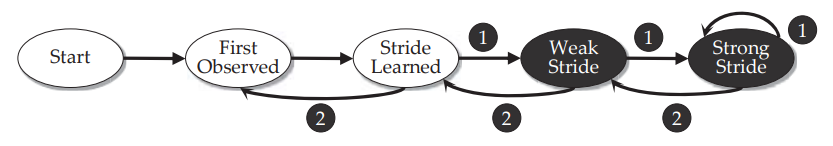
\includegraphics[scale=0.6]{stride-detector}
		\end{figure}
		
		This state machine keeps track of the stride length and position of previous accesses, inferring the stride length of the current access. The strong stride-weak stride states allow for short interruptions in otherwise consistent stride pattern. This may be helpful, for example, when accessing the rows of a two dimensional array. In this case, the access pattern may be unpredictable when switching between rows, but the overall stride pattern will remain the same. 
		
		\subsubsection{Data structure for non-strided accesses}
		
		Some memory access patterns are not strides. When this is the case, the SD$^3$ method calls these accesses "points", and puts them in a "point table", which is similar in structure to the pending and history tables in the naive method. These are kept separate from the strides, which are put in the "stride table". There is both a stride and a point table inside each history and each pending table. 
		
		\subsubsection{Data structure for strided accesses}
		
		Operations on non-strided accesses are efficient because the memory location of an access can be looked up quickly using hash tables. However, strides can conflict and be merged even when they don't start or end on the same address, so different data structures are needed. One possible method would just use a list of strides, but the pairwise comparisons needed to do conflict-check would take quadratic time. The SD$^3$ paper suggests use of interval trees to quickly prune the search space to mitigate this quadratic complexity.
		
		An interval tree is an augmented binary search tree that allows searches for intervals, instead of single values. An interval tree can efficiently find all intervals stored inside it which overlap with another interval. 
		
		Take the following tree below (WIKIPEDIA: \url{https://en.wikipedia.org/wiki/File:Example_of_augmented_tree_with_low_value_as_the_key_and_maximum_high_as_extra_annotation.png}), which stores 5 intervals, including \texttt{[20,30)}, \texttt{[10,15)}, and \texttt{[0,1)}. 
		
		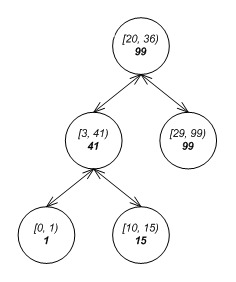
\includegraphics[scale=0.5]{interval-tree}
		
		This tree can be queried to find all intervals that overlap with another one, say \texttt{[40,50)} (this will return \texttt{[3,41)}, and \texttt{[29,99)}). Like a ordinary binary search tree, it is self-balancing and allows $O(\log(n))$ inserts and deletes. Finds are $O(m\log(n))$, where $m$ is the number of intervals it finds. 
		
		In the context of strides, each stride would simply be stored  an element in the tree keyed as an interval from first to last, inclusive. Then sets of strides will be looked up with efficiency relating to the total number of strides found, rather than the size of the set of strides. 
		
		\subsubsection{Merging strides}
		
		A simple way to MERGE two sets of strides is to join them together. However, this does not result in any compression. The online detection method generates strides for single accesses, which are immediately put in the pending table. So unless the adjoining strides in the history table are merged together with these strides during MERGE, the memory performance will not improve over the naive version. 
		
		Two strides are mergeable when they can be written as a single stride. For example \texttt{(first:1, last:10, interval:3)} and  \texttt{(first:13, last:22, interval:3)} can be merged, since the stride  \texttt{(first:1, last:22, interval:3)} covers the same elements as the two of them combined. On the other hand, \texttt{(first:2, last:8, interval:2)} and \texttt{(first:13, last:22, interval:3)} cannot be merged since simply extending the bounds of the stride cannot include all of the elements of both strides.
		
		SD$^3$ uses the interval tree described above to find possible candidates for mergable strides, and then checks further. If strides for a particular instruction are consistently not found to be mergable, then no further attempts are made to merge them. 
		
		\subsubsection{Finding overlap between sets of strides}
		
		During CONFLICT-CHECK, there are 3 different types of possible access conflicts: point-point, point-stride, and stride-stride. Point-point conflicts are found exactly as in the naive version, with hash table lookups. Possible point-stride and stride-stride conflicts are found using interval trees. Checking point-stride conflicts efficiently is simple, but checking stride-stride conflicts in constant time is more complex. 
		
		SD$^3$ introduces a new algorithm called Dynamic-GCD which efficiently finds overlap between strides. 
		To under how constant time stride overlap checking is possible, consider infinite length strides. Take two infinite length strides, with stride length $a$ and $b$. Take two points, one from each stride, and calculate the distance between them. Call this distance $c$. Then there is an integer $x$ and $y$ such that $ax + by = c$ iff the strides conflict. This condition is in turn equivalent to $c = 0 \mod (\gcd(a,b))$, where $\gcd(a,b)$ is the greatest common denominator of $a$ and $b$. This test can be done in constant time with the well known Euclidean algorithm for the GCD. Now, finite strides sometimes do not intersect when their infinite counterparts do, so the Dynamic-GCD algorithm gives a similar, but more complex test than the above that uses the Extended Euclidean algorithm to exactly compute intersection for finite strides. 
		
	\section{Bit compression}\label{s:bit-compress}
	
		A strided format is not the only method of compressing memory accesses. Memory accesses can also be compressed effectively using bit arrays. A bit array is simply an array of boolean variables which are stored inside individual bits, instead of in bytes, like ordinary C variables. 
		
		\subsection{Basis of bit compression}
		
		Stride compression is effective because many memory intensive procedures in real applications access memory in a strided fashion. Bit compression is effective because program memory is locally dense, meaning if memory is accessed in one location, nearby memory addresses are usually also valid program memory which will be accessed eventually. This property is virtually guaranteed by most modern operating systems, and so it is not as dependent on the program's structure as stride compression. 
		
		\subsection{Implementation of a bit compressed integer set}	
		
		A sparse set of integers is best implemented using a hash table. A completely dense set of integers is best implemented using a bit array. So a locally dense set will be implemented by a hash table where each item represents a fixed size set of memory. 
		
		
		
		
\chapter{Implementation}

	\section{Introduction to workload characterization}
	
		Workload characterization is a general technique to measure how applications use hardware features. Workload characterization uses dynamic analysis on a set of applications running on some set of hardware and collecting the runtime characteristics of the software. 
		
		Traditionally, hardware researchers are interested in the sorts of hardware characteristics that are important in application performance. They use workload characterization to understand how trade-offs in hardware design would affect various application's performance. To accomplish this, they collect metrics on the applications they want to optimize that are informative about the sorts of hardware trade-offs they are considering making. 
		
		We are interested in a related question: the application characteristics that can help the programmer choose between different established hardware platforms. We use workload characterization to understand the characteristics of single threaded CPU programs that are indicators of performance on other general purpose hardware, such as GPUs. We gathered applications and platform independent metrics that indicate important differences between the different hardware platforms. 
		
		\subsection{Important hardware characteristics under consideration}
		
		This thesis identifies several different hardware features as important, and attempts to capture in metrics. 
		
		\subsubsection{Scale of Parallelism}
		
		GPUs will not be faster than CPUs unless there is a high degree of parallelism, and substantial work to be done. GPUs have hundreds of cores, where CPUs at most two dozen or so. However, CPU cores are much faster. So GPUs will not be effective unless the work can be split over hundreds of threads. In addition, each kernel call must do substantial work, because the overhead of calling kernels is sometimes very high.  
		
		We suggest using the number of iterations in parallel loops, as well as the number of instructions each of those iterations contains to measure the scale of parallelism.
		% memory must be transfered back and forth between In addition, if the computation is extremely simple, say,  sometimes the cost of tran
		
		%GPUs are only useful when the algorithm can be divided into many threads, each of which has substantial content.
		
		%GPUs can run hundreds of threads have hundreds of are only useful when 
		
		
		\subsubsection{Predictability of memory accesses}
		
		
		GPUs have global memory that is optimized for high bandwidth and high latency. Predictable accesses such as strided memory can be streamed efficiently, while unpredictable memory accesses suffer from low latency, and stall the instruction pipeline. 
		%[CITATION???] possibly file:///C:/Users/weepi/Documents/thesis/papers/CCWS.pdf 
		CPUs are much better at handling unpredictable memory, since they have much larger caches. % also benefit from predictable memory accesses, but to a lesser extent, since the memory structure is optimized towards lower latencies. 
		
		We chose to capture this performance difference by measuring the number and length of strided accesses. 
		We use the same stride detector code as in our pairwise method (see section \ref{sse:stride-descr}.2 for an design). 
		
		% Then, we simply count the number of accesses which are of certain stride lengths, including zero length strides, and those that cannot be detected as strides. 
		
		\subsubsection{Parallelism Model}
		
		At a low level, GPUs execute threads in groups called warps. Warps have an SIMD (single instruction multiple data) model of execution, meaning that each thread in the warp executes instructions in lock-step. This implies that different threads in the same warp cannot execute different branch paths at the same time \footnote{\cite{Fung:2007:DWF:1331699.1331735}}. This performance hazard is called  branch divergence. Handling branch divergence is time consuming on GPUs, so performance suffers significantly when branch paths differ within a warp.
		
		Meanwhile CPUs have a MIMD (multiple instruction multiple data) model, where each thread executes code independently. CPUs are also equipped with advanced branch prediction which often reduces the cost of branches to nearly zero. 
		
		To account for this performance difference, we collected a count of the number of conditional branches encountered, and the number of time the path of that branch changed. 
		
		\subsubsection{Inter-thread vs Intra-thread memory sharing}
		
		CPUs theads have much larger cache capacity than GPU threads, since there are simply many more GPU threads active at a given time. \footnote{\cite{Jia:6835938}} This means that GPU threads cannot rely on caches to exploit temporal locality to the same degree that CPU threads can. Instead, GPU caches effectively exploit cross-thread locality. 
		
		To capture this, we measure the amount of memory shared between loop iterations vs reaccessed within a single iteration.
		We construct maps of the memory footprint of the loop and each of its iterations. From these memory footprints, we calculate the number of unique memory bytes accessed in each iteration as well whole instance. %From that, the number of shared bytes between threads 
		
%		
%		We capture this 
%		
%		CPU caches are designed to exploit temporal locality. If some piece of memory is accessed, and it is accessed again soon afterwards, the second access should be fast.
%		
%		
%		
%		These caches are quite large, typically 32kb for L1 cache, and 256kb for the L2 cache, so they allow for long temporal locality. 
%		
%		GPU caches and shard memory are not designed to capture long temporal locality. Caches are small, and are shared between many threads. 
%		
%		\footnote{\cite{Rogers:2012:CWS:2457472.2457487}}
%		
%		GPU caches 
%		
%		Global memory is expensive to access on both CPUs and GPUs. CPUs have a small number of cores, each with their own cache. These caches are optimized for temporal locality, i.e. the same memory being used across time.
%		
%		GPUs have hundreds of small cores, so they do not have their own cache. Instead, there are two different hardware features which both allow for fast access of memory which is shared across threads in a single timestep. One way is the shared memory, a different kind of memory in its own address space for local work-groups.
%		
%		the groups of cores have shared memory caches to allow for . 
%		
%		GPUs have shared memory and caches which allow for efficient cross-thread memory reuse assuming the shared data is reasonably small. 
%

		%\subsubsection{Arithmetic intensity}
	
	\section{Metrics}
		
		An important contribution of this paper is using a metric of parallelizability in workload characterization. 
		We created metrics in order to make use of this metric. 
		In particular, since we evaluate loop level parallelizability, we chose to collect all other metrics at the loop level. 
		
		We chose metrics based on the main differences between CPUs and GPUs. 
		
		\begin{tabular}{ |p{5.5cm}|p{8cm}| }
			\hline
			Metric & Relevant hardware characteristic(s) \\
			\hline \hline
			Number of iterations per loop instance & Scale of Parallelism \\
			\hline
			Length of loop iterations by instruction count & Scale of Parallelism \\
			\hline
			Number of writes/reads & ??? \\
			\hline
			Bytes accessed per instance & ??? \\
			\hline
			Total memory footprint of loop & Compare with Bytes for temporal locality?  \\
			\hline
			Shared memory footprint between loop iterations & Cross-thread spacial locality \\
			\hline
			Strided accesses  & Latency vs bandwidth \\
			\hline
			Number of branch changes & Warp divergence and branch prediction \\
			\hline
		\end{tabular}
	



	\section{Experiment design}
	
		To collect the 
		
		\begin{enumerate}
			%\item Run the workload natively to check native memory consumption
			\item Use LoopProf to evaluate the application's loop starts and ends
			\item Using those loop information, simulate the application again to collect the loop dependent metrics
			\item Using the same loop information, simulate the application while running a parrelleism detection tool to collect loop parrelleization information. 
		\end{enumerate}
		%		\subsection{Loop size metrics}
		%		\subsubsection{Number of iterations per loop instance}
		%		\subsubsection{Length of loop iteration by instruction count}
		%		\subsection{Memory metrics}
		%		\subsubsection{Number of reads/writes}
		%		\subsubsection{Bytes accessed per instance}
		%		\subsubsection{Total memory footprint of loop}
		%	
		
	\section{Workloads}
		
		To distinguish between applications that are best run on CPUs or GPUs, we first needed to get a good sample of programs with different characteristics. Some of these should be geared towards CPUs, and others should good cases for GPU acceleration. To get a wide variety of applications, we gathered applications from several different benchmarks: Rodinia, Parsec, and ..... 
		
		\subsubsection{Rodinia}
		
		Rodina is a benchmark designed to compare CPU and GPU performance on different applications. The Rodinia applications are chosen to reflect the Berkley 7 dwarves of scientific computation. \footnote{\cite{Che:2009}}
		
		\subsubsection{Parsec}
		
		\footnote{\cite{Bienia:2008}}
		
		Colella, Phillip. Defining software requirements for scientific computing. Slide of 2004 presentation
		included in David Patterson’s 2005 talk, 2004. URL http://www.lanl.gov/orgs/
		hpc/salishan/salishan2005/davidpatterson.pdf.
		\footnote{\cite{Che:2010}}
		
		
		
	\section{Stride Compression Implementation}
	
		The code that Kim et al. wrote to implement the SD$^3$ algorithm was not made publicly available, so it is closed source, and we cannot use it to detect parallelism. To achieve the goals of this thesis, we still needed to detect parallelism without running out of system memory, so we chose to implement the algorithm ourselves. As we had limited time to implement it, we decided to make changes to the algorithm for simplicity. In particular, we thought implementing interval trees ourselves would be error-prone, and we could not find an open source C++ implementation, so we chose to use other data structures. 
		In addition, the details of the Dynamic-GCD algorithm proved difficult to work out, so we used other techniques for finding stride conflicts.
		These were key features to ensure efficiency in the original SD$^3$ algorithm, so more changes had to be made to improve efficiency. In particular, a slow conflict-check method was used in our implementation, so optimizations were introduced that minimize the number of conflict-check operations that occur. 
		
		\subsection{Algorithm and data structure overview}
		
			%The key data structures and their use 
			
			First, a high level overview of the main data structures and objects will be introduced, and later the specific data structures and algorithms will be detailed. 
			
			At the highest level, a program has a single LoopStack, which contains a stack of LoopInstances. LoopInstances store all information about a particular active loop, including the pending and history tables.	Separate from the LoopStack, there is a StrideDetector for each instruction that accesses memory. 
			
			There are three main data structures which are central to the algorithm. The purpose of these data structures is outlined here, and the details will be explained later. 
			
			\begin{itemize}
				\item StrideTable: This table stores strided accesses and their instructions. Strides can be added efficiently to this table.
				\item PointTable: This table stores non-strided accesses and their instructions. 
				\item AddressSet: This structure is used as a set of memory addresses, without instructions. It has ordinary set operations, such as union, intersection, set subtraction, and inserting elements. It is used as an optimization only, as it stores strictly less information that the point and stride tables. 
			\end{itemize}
			
			These data structures store the content of the pending and history tables, but reads and writes are stored separately. See Figure \ref{fig:loopinstance} for how these tables fit inside the LoopInstance. 
			
			\begin{figure}[h]
				\caption{LoopInstance Layout}
				\label{fig:loopinstance}
				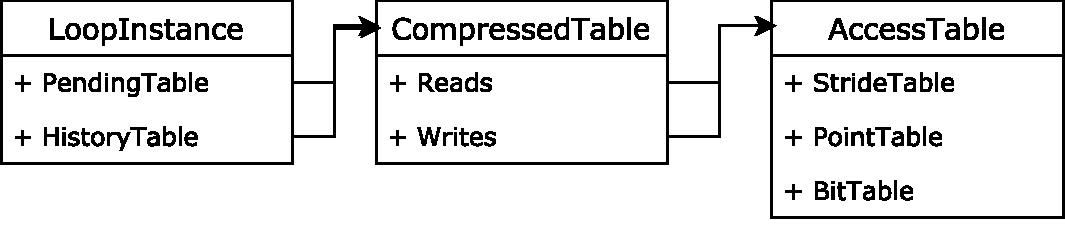
\includegraphics[scale=0.8]{LoopData.pdf}
			\end{figure}
			
			Given these data structures, new memory accesses are processed as described in Algorithm \ref{new-memory-acc}, loop iteration endings are described in Algorithm \ref{new-loop-iteration}, and loop termination is described in Algorithm \ref{loop-termination}.
			
			\begin{algorithm}
				\caption{New memory accesses}\label{new-memory-acc}
					When a memory location $m$ is accessed by instruction $i$, and LoopInstance $L$ is at the top of the loop stack,
					\begin{enumerate}
						\item If the memory location $m$ is killed by the pending table's AccessSet, do nothing, and skip the rest of the steps. 
						\item Find the loop-independent stride detector that corresponds to instruction $i$, and use it to calculate whether $m$ is a stride, and if so, its stride distance $d$. 
						%\item Get the point table, stride table, and AddressSet of LoopInstance $L$ corresponding to the accessmode of $L$.
						\item If $m$ is a stride with stride distance $d$ then add it to the appropriate stride table.
						\item If $m$ is not a stride, add it to the appropriate point table. 
						\item Add the bytes accessed by $m$ to the appropriate AddressSet.
					\end{enumerate} 
			\end{algorithm}
			
			
			\begin{algorithm}
				\caption{Finishing a loop iteration}\label{new-loop-iteration}
				When an iteration of loop $L$, with LoopInstance $I$ finishes,
				\begin{enumerate}
					\item Merge pending table contents into history table
					\begin{enumerate}
						\item Add every point and stride in the pending table into the corresponding point and stride tables of the history table
						\item Union the pending AccessSets into the corresponding history AccessSets.
						\item Clear the entire PendingTable.
					\end{enumerate}
					\item Check for conflicts between the pending and history tables
					\begin{enumerate}
						\item Determine if the iteration can be run in parallel by checking if the intersection of the pending table's read AccessSet and the history table's write AccessSet is empty.
						\item If the loop iteration is not parallel, find the pairs of instructions that conflict by
						\begin{enumerate}
							\item Get the list of all points/strides in the read pending table, and compare it the list of all points/strides in the write history table, and find a list of pairs of overlapping points/strides.
							\item Filter out the points/strides which are not actually conflicting.
						\end{enumerate}
					\end{enumerate}
				\end{enumerate}
			\end{algorithm}


			\begin{algorithm}
				\caption{Upon loop termination}\label{loop-termination}
				
				When loop $L$ terminates, with LoopInstance $I$ on the top of the LoopStack, and LoopInstance $I^\prime$ is the next highest on the stack,
				\begin{enumerate}
					\item Remove all strides and points from the history table of $I$ which are killed by the pending table of $I^\prime$.
					\item Merge history table contents into pending table.
					\item Pop $I$ off the LoopStack.
				\end{enumerate}
			\end{algorithm}
		
		\section{Adding accesses}
		
		
		
		\subsection{Stride Detection}
		
		The StrideDetector is implemented to match the original SD$^3$ design as closely as possible. The state machine matches Figure \ref{fig:stride-detector}.
		
		\subsection{Adding Points to the PointTable}
		
			Points (non-strided accesses) are added to the PointTable during new memory accesses and merges. The PointTable is designed so that redundant points are not duplicated in the table. 
			
			The PointTable is simply a set of Points keyed on instruction address and memory address see figure \ref{fig:point-table}. When a point is added, its location in the set is checked. If there is an element there already, nothing happens, otherwise the point is added to the set. 
			%Recall that Points are specified by instruction address, memory address, and access mode (read or write). 
			%In Figure \ref{fig:point-table}, you can see that the a Point is stored for each instruction and memory address. 
			
			\begin{figure}[h]
				\caption{Point Table}
				\label{fig:point-table}
				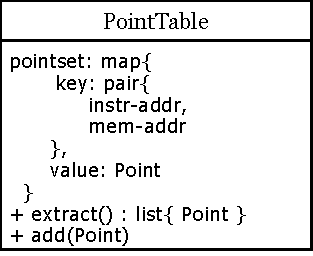
\includegraphics[scale=0.8]{point_data.pdf}
			\end{figure}
		
			
			%The data structures allow for a simple and efficient merge operation. The bit set is merged by an in-place union operation. For the point and stride tables, the operation simply calls \texttt{extract} to collect all the elements from the source table, and adds them one at a time to the destination table. 
			
			%The add operation is the only non-trivial operation. For points, it is straightforward: add the point if it is not yet there. This works because a point's location in the table uniquely specifies its value. 
			
			
		
		\subsection{Adding Strides to the StrideTable}
			
			Strides also added to the StrideTable during new memory accesses and merges. 			
			When possible, strides need to be merged into existing strides in the table when being added. This is critical for compression (see section \ref{sse:stride-descr}.5). The data structure is designed to make this process simple and efficient. 
			
			At a high level, the StrideTable is a unordered set of ordered sets of strides (see Figure \ref{fig:stride-table}). The outer set ensures that a particular inner set stores strides which are mergeable if they adjoin. The inner set is used to check if the strides do adjoin, in which case, they are mergeable.
			
			\begin{figure}[h]
				\caption{Stride Table}
				\label{fig:stride-table}
				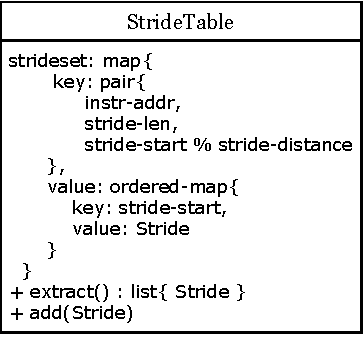
\includegraphics[scale=0.8]{stride_data.pdf}
			\end{figure}
			 
			
			As shown in Figure \ref{fig:stride-table}, the outer set is keyed on the instruction address, the stride distance, and the stride start modulo the stride distance. Strides which have these criteria in common are mergable if they adjoin, since These criteria ensure that all the strides in the inside set of strides which are all mergeable. 
			
			The inside set is ordered by the first element in the stride. Overlapping strides are always merged, there will never be overlapping strides in the set. This property will be used to guarantee efficiency.
			
			To see how this can be done, consider the below example, where there are 3 strides in the table, and one stride being added. Each grey block represents one stride: the added stride is six times longer than the other 3. The first stride cannot be merged with the added stride, and the other two can. 
			
			\newcommand{\bcl}{\cellcolor{black!50}}
			\begin{tabular}{ |c|c|c|c|c|c|c|c|c|c| } 
				\hline
				Current strides & \bcl &  & & \bcl & & &  & \bcl & \\ 
				\hline
				Added stride &  & & \multicolumn{5}{|c|}{\bcl} & & \\ 
				\hline
			\end{tabular}
			
			Since strides in the table will never overlap, the stride directly below the added stride is the only possible stride that starts before it, and also could overlap. In the example, it only has to check the one stride shown on the left. Then, it will merge every stride which starts after it starts, but ends before the added stride ends.
			
			%Two strides are possibly mergeable if they have the same instruction address, the same stride distance, the strides would be the same if they were infinite length. Referring back to Figure \ref{fig:stride-table}, these are exactly the strides which have the same value in the outer set, and so are placed in the same binary search tree. 
			
			%These criterion guarantee that any adjoining strides are mergable. The inner binary search tree is used to check if the strides do in fact adjoin. This is difficult because unlike an interval tree, only the start of the stride is ordered in the binary search tree.
		
		\section{Checking conflicts}
		
		\subsection{IsParrelel}
		\subsection{Find Overlapping}
		\subsection{Filter Non-conflicting}
		
		\section{Merge}
		
		\subsection{Killed bits}
			
		\subsection{AccessSet implementation}
			
			The AccessSet stores a set of memory addresses. This is in contrast to Point and Stride tables, which also store the instruction associated with each memory access. We found it necessary to store this separate table which stores strictly less information as an optimization. It is critical in reducing the number of inefficient Find-Overlapping operations that are needed. It is also helpful for quickly checking killed memory locations. 
			
			%In particular, it allows us to improve the performance of certain operations which do not need instruction information. 
			
			Since memory addresses are simply integers, we will discuss the implementation in generic terms of an integer set, rather than discussing memory addresses. To store this integer set efficiently, we use bit compression as discussed in Section \ref{s:bit-compress}.
			
			\begin{figure}[H]
				\caption{AddressSet data structure}
				\label{fig:bitset}
				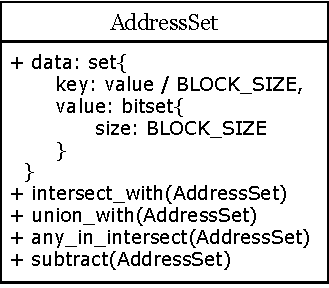
\includegraphics[scale=0.8]{bit_data.pdf}
			\end{figure}
			
			%The Bit table stores a set of overall memory accesses, independently of the instruction it was accessed.
			
			%Points and strides store which instruction accessed them. But some operations do not need that information, they only need the overall memory accesses in the scope, independently of the instruction. We found it advantageous to store this information as well. It is implemented as a compressed bit set, described loosely in section 1.6. Here is a more precise description of the set's data structure:
			
		
			Each of the operations are a combination of the obvious implementation for sparse sets, and the implementation for dense sets. Take in-place set intersection as a representative example. In a sparse set, in-place set intersection can be implemented by iterating through each element of the destination set, and deleting it if the element is not in the source set. In dense sets, the intersection is simply the boolean logical operation $x = x \land y$, applied to every bit. This can be implemented easily and quickly in C with the \texttt{\&} operator. Set intersection is implemented in the bit-set described above by treating the outer set as a sparse set, and the bit array as a dense set. See Algorithm \ref{bitsetintersect} for details. % going though each element of the source set, deleteing it is not in the destination set
			
			\begin{algorithm}
				\caption{BitSetIntersect}
				\label{bitsetintersect}
				\begin{algorithmic}[1]
					\Function{BitSetIntersection}{Dest,Src}
					
					\For{$\text{block},\text{bit-arr} \in \text{Dest}$}
					
					\If {$\text{blocknum} \in \text{Src}$}
					\State { Src.remove(blocknum)}
					\Else
					\State { bit-arr \texttt{\&=} Dest.get(blocknum)}
					\EndIf
					\EndFor
					
					\EndFunction
				\end{algorithmic}
			\end{algorithm}
			
			
			%The Bit table stores overall memory accesses, independently of the instruction it was accessed.
			%This is in contrast to Point and Stride tables, which do store the instruction associated with each memory access. We found it necessary to store this separate table which stores strictly less information for performance reasons. In particular, it allows us to improve the performance of certain operations which do not need instruction information. 
			
			
			%The Bit Table stores information about the memory accesses independently from the instruction at which it was accessed, whereas 
			
			
			%The LoopInstance object, which keeps track of all information for a loop, has separate tables for reads and writes
		
			%The data structures which implement point and stride tables are optimized for efficient merging, instead of efficient conflict checking. The details of their data structures will be explained when explaining merging. They have two methods, an "add" method, which simply adds an item to the table, and an extract method, which gets all current items in the table.
			
			
			%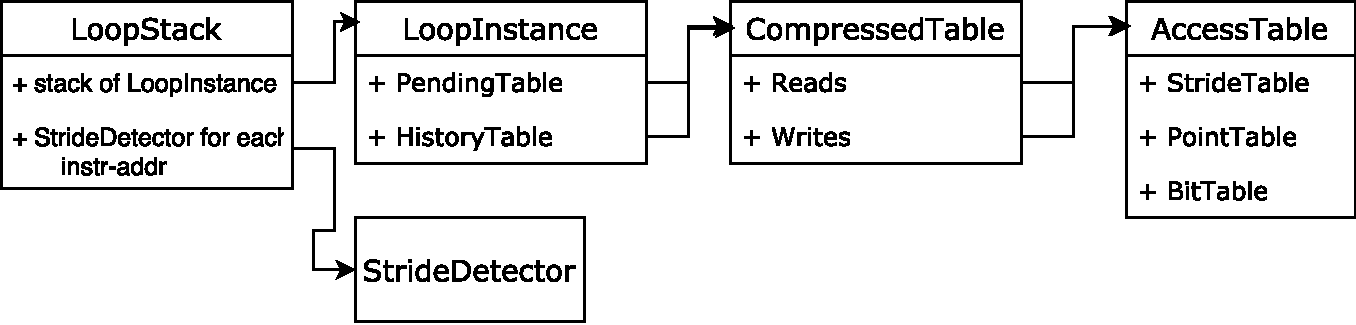
\includegraphics[scale=0.6]{FullLoopData.pdf}
			
		\subsection{Merge}
			The data structures which implement point and stride tables are optimized for efficient merging, instead of efficient conflict checking. They have two methods, an \texttt{add} method, which simply adds an item to the table, and an \texttt{extract} method, which gets all current items in the table.
			
%			
		\subsection{Conflict Check}

			In SD$^3$, there is a single procedure that evaluates memory conflicts. We broke CONFLICT-CHECK into two procedures for performance reasons. The first procedure, IsParallel, is a fast operation that simply checks the intersection of the bit sets of the reads of the pending table and the writes of the history table. It gives a binary answer, either the loop is parallel, or not. The second, slower operation, FindConflictingInstructions, finds the particular instructions which accessed the conflicting memory by looking at points and strides. Figure \ref{fig:conflict-check} shows the general outline of the relevant operations and data structures. 
			
			\begin{figure}
				\caption{Conflict-Check outline}
				\label{fig:conflict-check}
				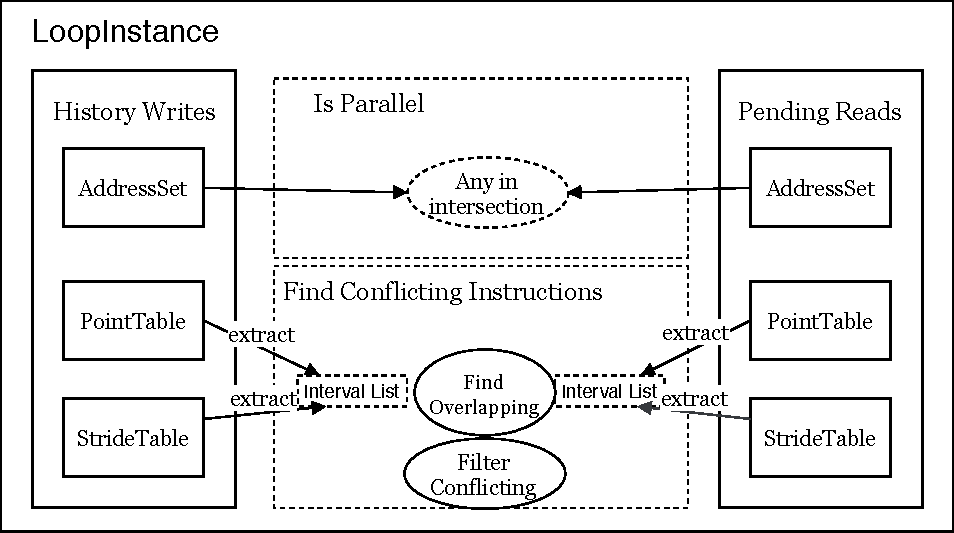
\includegraphics[scale=0.8]{conflict-diagram.pdf}
			\end{figure}
			
			
			Now, how does FindConflictingInstructions actually work? Similarly to SD$^3$, it is broken up into two steps. First, lists of strides and points are gathered by using \texttt{extract}. Then, these strides and points are treated as intervals, and the intervals that overlap are found in FindOverlapping. Finally, whether the strides and points actually overlap is calculated in FilterConflicting.
			
			\subsubsection{Find Overlapping}
				
				FindOverlapping uses a sliding window technique on sorted lists of intervals to compute a list of pairs of overlapping intervals. Call these lists A and B. The algorithm first sorts the two lists of intervals by their start. It considers each interval from A one at a time, call this interval $I$. It keeps a window of intervals of list B which overlap the start of $I$. Each time another interval from A is checked, the algorithm it drops the intervals which end before the new interval starts, and adds in all the intervals which start before the new interval starts, but end after it starts. Then it finds the intervals from B which start after $I$ starts, but before $I$ ends. Algorithm \ref{algo:findoverlapping} has psuedocode for this algorithm.
				
				\begin{algorithm}
					\caption{Find Overlapping}
					\label{algo:findoverlapping}
				\begin{verbatim}
				find_overlapping_intervals(A,B)
				    sort A by first()
				    sort B by first()
				    overlap = Set()
				    before_last = vector()
				    ib = 0
				    for interval in A
				        new_before_last = vector()
				        for item in before_last:
				            if item.last() >= interval.first():
				                new_before_last.append(item)
				        swap(before_last,new_before_last)
				
				        increment ib until B[ib].first() >= interval.first()
				        
				        if B[ib].last() >= interval.first()
				            before_last.append(B[ib])
				
				        for bl in before_last
				            overlap.add(bl,interval)
				
				        for ib2 from ib until B[ib2].first() > interval.last()
				            overlap.add(B[ib2],interval)
				\end{verbatim}
				\end{algorithm}
			
			\subsubsection{Filter Conflicting}
		
				Recall that the SD$^3$ paper uses the efficient Dynamic-GCD algorithm. We found it difficult to work out the details of this algorithm, so instead, we decided to use other methods. In particular, the vast majority of strided conflicts will be much easier to check. Many strides will be dense, every byte in between the start and end will be accessed. Many other possible conflicting strides will have the same stride distance. And most of the remaining strides will have long interval overlap compared to the stride distance, which means that the ordinary GCD test gives the correct answer.
				Our method simply checks if these cases apply, and if so, calculates the answer. The few remaining cases can be checked with a slow algorithm which compares the strides element by element.
				 
				%In particular, it is important to note that having constant time comparison is not needed for algorithmic efficiency of the method. After all, each element of the stride is added one at a time, and it is only compari
				
			%Instead of using interval trees, we used data structures optimized towards merging strides and points. Points can only be merged if their instruction and memory address is the same, so they are stored by instruction and memory address. 
			
			\subsubsection{Truncated execution of FindConflictingInstructions}
			
			Because FindConflictingInstructions is a slow operation, it should be run as infrequently as possible to collect the information we need. Our method only runs it a constant number of times for a particular loop instance. This is made possible by two observations:
			
			\begin{enumerate}
				\item If the loop iteration does not have any conflicts (discovered by running IsParallel), then we know that no instructions have conflicts, so we do not need to check them. 
				\item  The conflicting instructions are simply guides to the programmer. As such they do not have to be 100\% accurate. In particular, if there are some instruction conflicts which are reported, and others which are not, this is not a serious problem. So this information can be truncated.  
			\end{enumerate}
			
			These two observations give rise to the following procedure, which ensures that the FindConflictingInstructions() is only run a constant number of times:
			
			\begin{algorithm}
				\caption{CONFLICT-CHECK}
				\label{conflict-check}
				\begin{algorithmic}[1]
					%\Function{RecursiveSum}{A,s,e}
					\If {$\textsc{IsParallel(H,P)}$}
					\State Report parallel iteration 
					\ElsIf{ConflictingIters $>$ TRUNCATE-OUTPUT-ITERS}
					\State Report not parallel iteration 
					\Else
					\State InstrInfo = $\textsc{FindConflictingInstructions(H,P)}$
					\State ConflictingIters \texttt{+=} 1
					\State Report not parallel iteration with conflicts: InstrInfo
					\EndIf
				\end{algorithmic}
			\end{algorithm}
		
		\subsection{Subtract Killed}
			
			The SD$^3$ algorithm subtracts killed points and strides by a similar algorithm to their conflict-check method. We used the bit sets to do this instead. After all, killed bits are most easily described using the bit sets. We simply used the bit sets to check whether points and strides were killed or not one at a time. To guarantee runtime efficiency, the elements of a stride are checked one at a time, starting from the front of the stride, and one at a time. This process terminates at the first stride element that is not killed. 
		
		
	\section{Bit Compression Implementation}
	
		
	
	\chapter{Results}
	
	\section{Intro}
	
	
		\begin{tabular}{ |p{5.5cm}|p{8cm}| }
			\hline
			Metric & Relevant hardware characteristic(s) \\
			\hline \hline
			Number of iterations per loop instance & Potential for massive parallelism \\
			\hline
			Length of loop iterations by instruction count & Potential for massive parallelism \\
			\hline
			Number of writes/reads & Memory bandwidth??? \\
			\hline
			Bytes accessed per instance & Memory bandwidth??? Compare w/Footprint for temporal locality? \\
			\hline
			Total memory footprint of loop & Compare with Bytes for temporal locality?  \\
			\hline
			Shared memory footprint between loop iterations & Cross-thread spacial locality \\
			\hline
			Strided accesses  & Latency vs bandwidth \\
			\hline
			Number of branch changes & Warp divergence and branch prediction \\
			\hline
		\end{tabular}
		
		
	
	
		\begin{tabular}{ |l|l|l| }
			\hline
			Application          & Suite   & Input  \\ \hline
			\hline
			B+tree & Rodinia  &     \\ \hline
			Back Propagation & Rodinia  &    \\ \hline
			Breadth First Search & Rodinia  &    \\ \hline
			CFD & Rodinia  &    \\ \hline
			Heartwall & Rodinia  &   \\ \hline
			Hotspot & Rodinia  &    \\ \hline
			Hotspot3d & Rodinia  &    \\ \hline
			kmeans & Rodinia  &     \\ \hline
			lavaMD & Rodinia  &     \\ \hline
			leukocyte & Rodinia  &     \\ \hline
			LU Decomposition & Rodinia    &  \\ \hline
			Myocite & Rodinia  &     \\ \hline
			Nearest Neighbor & Rodinia  &     \\ \hline
			Needleman-Wunsch & Rodinia  &     \\ \hline
			ParticleFilter & Rodinia  &     \\ \hline
			PathFinder & Rodinia  &     \\ \hline
			SRAD & Rodinia  &     \\ \hline
			StreamCluster & Rodinia  &    \\ \hline
		\end{tabular}
	
\chapter{chpt2}
		%\subsection{Bit compression}
		
		%Another possible compression method is by using a 
		
			
	\section{Motivation}
	
		Recall that one of the most important things to establish about the program is whether it can in theory run in parallel. This is a very important factor in determining a program's hardware matchup.

		One problem is that there are no good open source tools for determining theoretical parallelism in real code. So we will have to create one ourselves. We will constrain ourselves to loop parallelism, as detecting general parallelism is impossible. 
		
		To help explain the algorithms and data structures involved, I will bring in a couple of code examples in order to show how the algorithms work. 
		


	\section{Data Dependency graphs}
		So how might you detect parallelism? To do that, you have to have a mathematical model of what parallelism is.

		Our model is a data dependency graph.

		The idea is that we can take a computation and build a directed acyclic graph like so.

		The inputs to the computation are nodes $I \subset V$. These can be thought of as blocks of memory stored before the computation starts. Each step of the computation produces a temporary value $c \in V$. There is an edge $(u,v)$ whenever an input to $u$ is the data calculated by $v$. Then some nodes are designated outputs, which are the data we wished to calculate.

		This is a directed acyclic graph because in a computation, no sub-computation can use data that hasn't been calculated yet, including the data output by its own computation.

		For example, you can break the computation of $A+B+D+A\times B$ into a few steps like this

		\begin{algorithmic}[1]
			\State $D \gets A+B$
			\State $E \gets A\times B$
			\State $F \gets D+C$
			\State $G \gets E+F$
		\end{algorithmic}

		And then use these sub-operations to build the following dependency graph.

		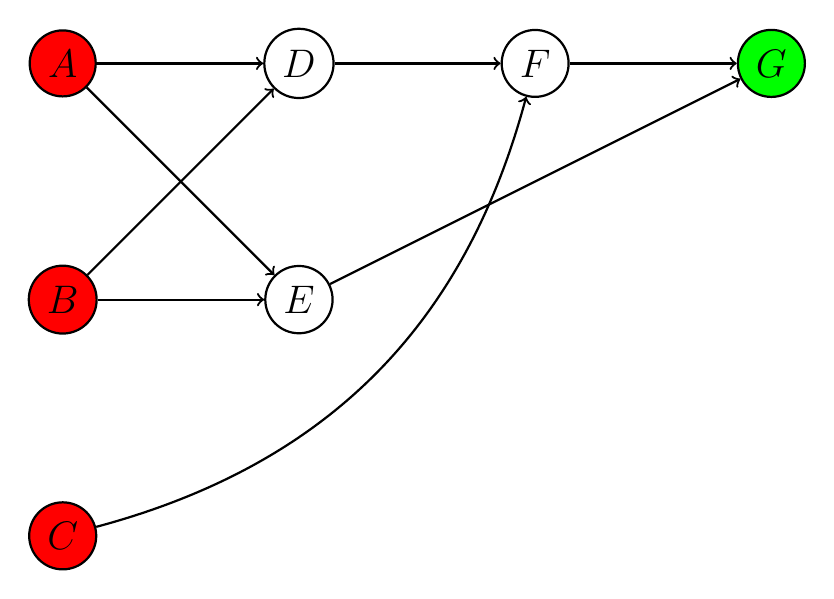
\begin{tikzpicture}[auto, node distance=3cm, every loop/.style={},
		thick,main node/.style={circle,draw,font=\sffamily\Large\bfseries}]

		\node[main node] [fill=red] (A) {$A$};
		\node[main node] [fill=red] (B) [below of=A] {$B$};
		\node[main node] (C) [right of=B] {$E$};
		\node[main node] [fill=red] (D) [below of=B] {$C$};
		\node[main node] (F) [right of=A] {$D$};
		\node[main node] (E) [right of=F] {$F$};
		\node[main node] [fill=green] (G) [right of=E] {$G$};

		\path[every node/.style={font=\sffamily\small}]
		(A) [->] edge node [left] {} (C)
		(B) [->] edge node [left] {} (C)
		(A) [->] edge node [left] {} (F)
		(B) [->] edge node [left] {} (F)
		(F) [->] edge node [left] {} (E)
		(E) [->] edge node [left] {} (G)
		(C) [->] edge node [left] {} (G)
		(D) [->] edge [bend right] node [left] {} (E);
		\end{tikzpicture}

		Hopefully you can see that this is an intuitive framework to examine parallelizability In the example above, nodes $D$ and $E$ can be run in parallel since neither depend on the other. $F$ can also be run in parallel with $E$, but not with $D$, since it depends on $D$ already being calculated. $G$ can only be run after all other steps are finished, as it recursively depends on $D,E$, and $F$.

		The degree to which this graph is parallelizable corresponds to the depth of the graph. By depth, we simply mean the maximal length of any path from an input to an output. This can be easily calculated using topological sort. This maximal length is guaranteed to be finite for any directed acyclic graph. In the example above, the depth is 3, as $A\rightarrow D \rightarrow F \rightarrow G$ has 3 edges, and no path has more than 3.

		The most important kind of parallelism, and the only kind we will care about is massive parallelism. Massive parallelism is defined to be any computation where the depth of the dependency graph is logarithmic in the size of the input.

		One extremely simple example of a massively parallel algorithm is a vector addition. If you want to sum two vectors $a$ and $b$, by computing $c = a+b$, then the obvious algorithm is to take each $i$, and compute $c_i = a_i + b_i$. Since each of these operations is completely dependent on the others, this is a constant depth dependency graph.

		One important example of a massively parallel algorithm is summing. When you have an array $A_1,A_2,...,A_n$ of numbers and you sum them, there are different ways to do it, some of which are parallelizable, some of which are not. The most obvious sequential algorithm, computing $(A_1+(A_2+(A_3+...+A_n)))$ has a dependency graph of depth $n$. However, addition is associative, so we can rearrange the parenthesis like this: $(((A_1+A_2)+(A_3+A_4))+...(A_{n-1}+A_n))$ to give us a log depth dependency graph. Below are two algorithms that describe these methods.

		\begin{algorithm}
			\caption{MassiveParrelelSum}\label{parellelsum}
			\begin{algorithmic}[1]
				\Function{RecursiveSum}{A,s,e}
					\If {$e - s \le 2$}
						\Return {$\textsc{StandardSum}(A[s:e])$}
					\EndIf
					\State $m \gets \floor{e-s}$
					\State $s_1 \gets \textsc{RecursiveSum}(A,s,m)$
					\State $s_2 \gets \textsc{RecursiveSum}(A,m,e)$
					\State \Return $s_1+s_2$
				\EndFunction
				\Function{StandardSum}{A}
					\State $s \gets 0$
					\For{$a \in A$}
						\State $s \gets s + a$
					\EndFor
				\EndFunction
			\end{algorithmic}
		\end{algorithm}

		Now, this is bad since we have two algorithms to compute the same problem, but one of which is parallelizable, and one of which is not. And what allows us to do the transformation from one to the other depends on an algebraic quality that is true for many operations and procedures other than addition. For example subtraction is not associative, but repeated subtraction can have a similar transformation because you can take $\text{RepeatedSubtraction}(A) = -\text{Sum}(A)$, and then do the same log depth calculation with only one more step at the end.

		This general method of using divide and conquer to turn a linear depth operation into a log depth one is called a reduction, and is the basis of the MapReduce cluster computing paradigm.

		Since these are important targets of parallelization, we will try our best to identify these cases, but it is most likely impossible to assess the possibility of this transformation automatically with perfect accuracy, so we will have to analyses actual cases.

		\subsection{Reporting}

		Just detecting a binary "is parallel" or "is not parallel" is not particularly useful. If it is a small loop, then it is easy to see if it is parallel or not by hand. A larger loop in real code is quite unlikely to have no data dependencies at all, and so they will rarely be parallel. If the parallelism detector says a larger function is not parallel, then the analysis you do with it won't know if the part that is not parallel is important or not. It could be an assert or logging that is non-vital, or perhaps something that can be pulled out of the loop. However, it is difficult to automatically detect such things, but instead, we can report what in the loop is stopping the function from being parallel to a human. A human, one shown where the problems are, may be able to tell  And a human using this tool won't know where the problem is, and may take a lot of work to find this issues, unless the code tells the human where to look. The most useful information is what instruction the conflicts are coming from, but there are others, for example, the memory location, and the number of accesses which conflict.

		The number of times conflicting accesses happen is useful for us because it gives some indication as to how well it were to perform if we had some sort of locking mechanism serializing accesses to the bit of memory.

		Because this is not the main point of the thesis, I will focus on making a good attempt to report the instruction locations of the conflict, and the number of times conflicts happen. But perfection is not necessary here.

		\subsubsection{Reporting List}
		\begin{enumerate}
			\item Whether a loop is parallel
			\item Number of bytes that conflict between iterations
			\item Instructions that conflicts
			\item etc.
		\end{enumerate}

	\section{Pairwise method}

		Note that any naive implementation of actually constructing a data dependence tree from a real computation will take $\Omega(n)$ space, where $n$ is the number of steps of the computation. Even for quick computations, this memory requirement quickly grows beyond RAM capacities of normal machines, and analysis becomes unusably slow. So instead, we will look at special cases and approximations to get what we need.

		The pairwise method is a approximation of data dependence analysis which has been developed to examine loop level parallelism.

		\subsection{Terminology}
		\begin{itemize}
			\item Loop iteration
			\item Loop instance
		\end{itemize}

		\subsection{Idea and inspiration}

		Loop level parallelism is when one iteration of a loop is independent from the rest. This kind of parallelism is the main target of massively parallel architectures. Other types of parallelism, including parallel recursive calls and task parallelism are generally less important or less parallelizable than loop level parallelism.

		The idea is to figure out if an iteration of a loop is independent from each other loop iteration. If this is the case, then it clearly is highly parallelizable

		The real reason why this is an important case is because it is very easy to measure, requiring very little memory and computation. Take the following loop:
\begin{lstlisting}
for(int i = 1; i < n; i++){
	//operation 1
	//operation 2
	//operation 3
	//...
}
\end{lstlisting}


		To check if this code runs in parallel, we only need to keep track of two things:

		\begin{enumerate}
			\item Which memory addresses have been written and read in the current loop iteration. Call this the pending table.
			\item Which memory addresses have been written and read in all of the previous loop iterations in the same instance. Call this the history table.
			\item Which memory addresses in the current loop iteration that their first access was a write. Call this the killed addresses.
		\end{enumerate}

		So int the example above, say we were at operation 2 in iteration 30. So in other words, $i=30$, and we have executed operation 1.

		Then we only need to keep track of which memory addresses were read and written in operation 1 in the current iteration, and the reads and writes of all the operations in each previous iteration, i.e. when $i < 30$.

		So instead of having a memory requirement that scales with the size of the number of operations in the code, we have a memory requirement proportional to the amount of memory that the original app uses times the number of nested loops.

		\subsection{Implementation}

		The algorithm itself is quite simple:

		You just need 4 core operations, and the rest is straightforward:

		\begin{enumerate}
			\item Add a new memory access to the pending tables, considering killed bits of current loop iteration
			\item Merge in the historytable from a nested loop into the pendingtable of the current loop. When doing so, remove the killed addresses, and add the addresses that have been written to the killed addresses set.
			\item Merge in pending table into history table, finding access conflicts between the two.
		\end{enumerate}

		\begin{algorithm}
			\caption{Pairwise-Method}\label{pairwise-method}
			\begin{algorithmic}[1]
				\State When you see a new loop, push it on the loop stack
				\State On memory access, \textsc{ADD}
				\State On loop iteration end \textsc{MERGE PEND HIST}
				\State On loop instance end \textsc{MERGE HIST PEND}
			\end{algorithmic}
		\end{algorithm}

		\subsection{Correctness}

		To prove that this always produces a correct answer to the problem, consider the each loop iteration to be a single computation in the graph. The memory addresses that are reads first are clearly inputs to this operation, and the output are writes. Memory addresses that are written before being read are not inputs, and so should not be counted as such.

		So if any write of one iteration is read by another, then clearly, this dependency graph is not 1 depth, as the output of one operation is the input of another.

		If the dependency graph is depth 1, then this means there was no reads of any data that was output in other iterations.

		So this method works if every loop is independent from every other loop.

		Unfortunately, this method does not guarantee any good results if there is any dependence whatsoever in between loops for example, the following loop has a dependency graph depth of two.

\begin{lstlisting}
for(int i = n; i < 3n; i++){
	A[i] = A[i-n]+1;
}
\end{lstlisting}

		To see why its dependency graph is so small, note that you can simply break this into two loops, one from $i = [n,2n-1]$, and $i=[2n,3n-1]$, and in both loops, simply compute the answer in parallel.

		However, the pairwise method simply returns that all of the iterations after $i \ge 2n$ are not parallelizable, as they conflict with the memory addresses in some previous iteration. This is a direct consequence of the memory saving property of the pairwise method, so this problem is not solvable by this method.

		\subsection{Collecting additional information}

		As mentioned before, we will want not only report a binary parallel/not parallel, but also collect some fairly substantial additional information. In particular, we care about which instruction the dependencies came from.

		So in addition to storing information about which memory accesses are reads and writes, we will also need to store the instruction each read and write came from. One way to implement this is to store a set of memory reads and writes for each instruction.
%\begin{lstlisting}
%for(int i = 0; i < n; i++){
%	B[i] = A[i-1];
%	A[i] = C[i];
%}
%\end{lstlisting}

		\subsection{Registers and Flags}
		Unfortunately, memory locations are no the only source of possible memory dependencies. There are also registers.


		One case of a unparallelizable register/flag dependency is multiprecision addition.

		Say you have 2 numbers of arbitrary size, $A0$, and $B$. $A_i$ is the $i$th 64 bit block of $A$. Then you have the following algorithm to compute addition:

		\begin{lstlisting}
cary = 0
for(int i = 0; i < min_size(A,B); i++){
	R[i] = A[i] + B[i] + cary;
	if(register_overflowed(A[i] + B[i] + cary)) {
		cary = 1
	}
	else{
		cary = 0
	}
}
...
		\end{lstlisting}

		The first thing to note is that in the worst case, you cannot write to any element of $R_i$ before reading every element of $A$ and $B$ before $i$. So it is not parallelizable in this case. In practice, it will be somewhat parallelizable, since that case can safely be assumed to be rare. But a memory-only pairwise method will see that this loop is trivially parallelizable On the other hand, looking at the registers, there is a clear read-after-write conflict.

		Some papers ignore this case, as register dependencies can be analyzed statically.\footnote{\cite{Chen:2004}} However, for our uses, we need to know about register dependencies, and so we need to do this either statically or dynamically.

		Static analysis would mean introducing new tools to our project, and even static analysis may yield false negatives of parallelism (due to branching dependences).

		Dynamic analysis of registers could be easily implemented as a special case of memory dependence, as registers can just be considered another type of memory. However, registers are changed far more often than memory, and so we would need to do things somewhat differently if we don't want to suffer a large performance hit.

		So we need to make some kind of tradeoff here. I think the right choice is to do dynamic dependence analysis, but keep it somewhat separate from memory dependence analysis.


		\subsection{Memory/Performance issues}

		Unfortunately, a naive implementation of the pairwise method can consume hundreds of times more memory than the executable code.

		Each loop needs its own copy of all the accesses made by every instruction. This could mean in theory a $cmn$, where $c$ is the number of bytes needed to store the relevant info, (say 20, at least), $m$ is the number of instructions, and $n$ is the number of bytes of memory used by the executable program. Then we also need to store the instruction of each access, which makes it worse.
		
		Now, a naive hash table based method has a single entry for every access. 
		So $$O(M)$$. Even a highly optimized version will have at least 100 bits of overhead, and an unoptimized version will have much more, probably around 150-300, depending on hash table implementation and other details. 

		Of course, in practice it is quite a bit more efficient than this, since not every instruction will access every byte of memory, but it will still take up more memory than most computers can hold just to run basic benchmarks. \footnote{\cite{Kim:2010}}

	\section{Stride compression}

		A solution to the memory problems of the pairwise method is stride based compression. The SD3 paper lays this out in some detail \footnote{\cite{Kim:2010}}

		\subsection{Goals of compressed algorithm}
		The goal of any compression algorithm of this setting is to compute the basic steps of the pairwise method as accurately and quickly as possible, without using excessive memory. The time performance goal will means that we want a method that does not involve decompression if possible, as operating on compressed structures promises to be faster than decompression.


		\subsection{SD$^3$ method}

		\subsubsection{Stride detection on new memory accesses}

		When a memory address is accessed, the program decides if the access is part of a stride using an an on-line algorithm. If that algorithm returns true, then a singleton stride is immediately put in the stridetable.

		\subsubsection{Compressing/merging strides}

		As singleton strides are the only kind being added to the stridetable directly, then we really need a way to join these strides together.

		This is done using another interval tree at the instruction level.


		\subsubsection{Finding overlap}

		To

		\subsubsection{Killed points and strides}

		%\subsection{SD3 data structures}

		%Is this really needed?

		%\subsubsection{PC table of interval trees for merging}
		%\subsubsection{Memory interval tree for conflict-checking and address killing}

		%In general, the history table and the pending table are one type: call this the CompressedAccessTable type

		%In SD3, this is split in two different tables, a StrideTable for strides, and one for accesses which do not follow a stride pattern. Call these non-stride accesses points, and the table which stores them the PointTable.

		%The StrideTable is a conceptually a set of strides for each instruction. To accelerate detecting conflicts, there is a connected structure that is an interval tree linking to each stride, instruction pair.

		%The PointTable is a set of instructions at each memory address that has been accessed.

		%Note that while both tables enough information to get pairs of addresses, and the instructions involved, they have quite different performance characteristics, optimized to fit certain data structures, and the operations described below.

		\subsection{My Stride compression method}

		Stride detection on new memory accesses is the same. Finding overlap between two different strides is basically the same (except doesn't use dynamic-gcd).

		\subsubsection{Compressing/merging strides}

		Here we use a totally different data structure for stride merging.
		\begin{verbatim}
		unordered_map<instruc_addr,
		    unordered_map<pair<stride_len,access_size>,
		        map<stride_start,Stride>>>
		\end{verbatim}
		This is the data structure that is held at all times in the pending and history table.

		And then the obvious algorithm to add in new strides, while combining that with overlapping or adjacent strides with same instruction, stride-len and access-size.

		Unlike SD3, this data structure will always merge mergable strides, so there is no need for caching results.

		\subsubsection{Finding overlap}

		Unlike SD3, Strides and Points are both treated as intervals when finding overlap (in SD3, points are memory locations in a hash table).

		When finding exact overlap between history tables and pending tables, it builds a sorted list of points and strides.

		Then it does interval checking using the following linear time algorithm:

		\begin{verbatim}
		check_overlap(A,B)
		    sort A by first()
		    sort B by first()
		    overlap = Set()
		    before_last = vector()
		    ib = 0
		    for interval in A
		        new_before_last = vector()
		        for item in before_last:
		            if item.last() >= interval.first():
		                new_before_last.append(item)
		                swap(before_last,new_before_last)

		        increment ib until B[ib].first() >= interval.first()
		        if B[ib].last() >= interval.first()
		            before_last.append(B[ib])

		        for bl in before_last
		            overlap.add(bl,interval)

		        for ib2 from ib until B[ib2].first() > interval.last()
		            overlap.add(B[ib2],interval)
		\end{verbatim}

		\subsubsection{Killed points and strides}

		Written, read, and killed addresses are kept track via a single loop level compressed bit-set. Merged points and strides are compared with this map in order to eliminate killed accesses.

		Points and strides are not guaranteed to be killed if only part of the memory region they cover has been killed.

		\subsection{Bad cases of stride compression}

		Doesn’t really work on all code/workloads (need backup system that works decently)

		Examples:

		Graph computations (simulations, network analysis)

		Non-trivial data structures (BST, hash tables)

		%\subsubsection{More general access compression?}

		%The innermost loop may not have striding access, but the non-striding access may be similar to its own behavior in a previous iteration of a larger loop (for instance in a graph computation where it iterates over all the edges of a vertex in each iteration of a loop).


		%Idea: We can see all accesses of data as the set of permutations of memory addresses. We know that there are patterns in accesses. We can make a general purpose compression of memory accesses, where the stride compression is a special case of.

		%Trick: We need to somehow do efficient computations on these things.

	\section{Stride compression}

		\subsection{Examples of different kinds of strides}
		The most common and important kind of stride is accessing every element of standard array. This can be a dense stride, if you are accessing the entire element. But often, you have a array of structs, and you are only accessing part of the struct in the loop. This is a $ $

		The other main kind is going along an axis of an $n$-dimensional grid.

		But there are other kinds of stride accesses. For instance: diagonals on an $n$-dimensional grid (bishop movement in chess). Or linear derandomization, like in linear open hashing.

	\section{Stride based dependency checking on normal access patterns}

		Lets say we have 2 strides in the form $[ax+c]$ for $0\le x \le \alpha$, and $[by+d]$, for $0 \le y \le \beta$. We want to quickly and efficiently check if there is a dependency, and if so, then where they are.

		GCD negative check: If $|d-c| \ne 0 \mod \gcd(a,b)$, then there is no dependency. Intuitively, this is true because if the difference between the strides is a value that cannot be taken by combinations of $a$ and $b$, then there can never be an overlap.

		Interval Overlap Check: If intervals $[c,a\alpha+c]$, $[d,d+b\beta]$ do not overlap, then there is no dependency.

		In order to have a positive check for dependencies, and to count the number of dependencies, there is a little more you have to do, but it can still be done efficiently.

		\subsection{Handling different sized blocks}

		Unfortunately, things are more complicated then they might seem just looking at the above.
		The reason is that hardware allows memory accesses of varying bytes on the same data. For example, you might examine a text one byte at a time, and then later examine it in 8 byte blocks. Even worse, common hardware does not force aligned access. So there might be a 4 byte access with stride length of 12 bytes, starting from 3, and a 8 byte access of 16 stride length starting from 7. So we need to introduce another concept to stride checking in order to make this work: block size.

		There is an efficient way of finding if there is an dependency, assuming strides length is a multiple of block size for all strides. And we can just make our stride detector only detect strides like this.

		But how do we find the exact number of dependencies and where they are? What do we do about killed bits in this context (since this can lead to really awkward strides)?

		So instead of carefully dealing with abnormal strides like this slowly and carefully, I will instead just make basic checks, and then assume the worst case, whatever that may be in this context.

	\section{Bit set compression}

		Now, instead of using the common paradigm of strides to compress data, there is another way:

		\subsection{Bit-compressed set design}

		A process's allocated memory locations are sparse across the 64 bit address space, but dense locally. To take full advantage of that, the set is a map (binary search tree) of the different upper 56 bits that are accessed, and if a particular value is  the value any bits set in the lower 8 bits are stored in a bitmap.

		so really

		\begin{verbatim}
		map<upper_56,bitmap<256>>
		\end{verbatim}

		I will call the bitmaps blocks.

		\subsection{Note on performance of BSTs vs Hash tables}

		I ended up with BSTs rather than hash tables because of two reasons
		\begin{enumerate}
			\item BSTs tend to be faster on extremely small sets, like of size 1 or 2. This is important for the algorithm on inner loops.
			\item BSTs allow intersect checking in linear or sub-linear time in common cases.
		\end{enumerate}

		Efficient algorithm to check if there is anything in the intersection of the sets.
\begin{lstlisting}
bool CompressedSet::has_any_in_intersect(CompressedSet & outer){
	for(set_iterator iter = this->data.begin(), outer_iter = outer.data.begin();
	iter != this->data.end() && outer_iter != outer.data.end(); ){
		int64_t this_key = iter->first;
		int64_t outer_key = outer_iter->first;
		if(this_key == outer_key){
			BlockSet block = iter->second;
			block &= outer_iter->second;
			if(block.any()){
				return true;
			}
			++iter;
			++outer_iter;
		}
		else if(this_key < outer_key){
			iter = this->data.lower_bound(outer_key);
		}
		else{
			outer_iter = outer.data.lower_bound(this_key);
		}
	}
	return false;
}
\end{lstlisting}
		Efficiency (worse case $O(n\log(n))$ time, best case $O(\log(n))$ time, dense in both sets $O(n)$ time.


	\subsection{Bit-Compressed Conflict-check algorithm}

		\subsection{General idea}

		The existence of this bit based compression begs the question: Can we use this method to compress data more effectively than the SD3 style stride compression?

		In order to track down dependencies, we need a mapping between the reads and writes, and which instructions they were queried at.

		The natural way to represent this with compressed sets is to have a different set for each instruction. Assuming each instruction has many memory locations, which are reasonably close to each other, this promises to be quite efficient. The only problem is to efficiently find conflicts between different instructions.

		\subsection{Implementation}

		While the code is quite simple (the main source file is under 200 lines of c++), the ideas are a little unusual.

		\begin{verbatim}
    \begin{verbatim}
    The idea is this:

    For compressed memory access, we want 3 things

    2 sets of instructions, each with a set of memory locations they accessed

    You want to be able to

    1. Merge these together
    2. Find instructions that have overlapping memory addresses


    There are other operations involving a single set such as

    1. Remove all bits that are in a set of adresses
    2. Find the union of all memory adresses

    In order to accomplish all these things efficiently, we be constantly relying on the
    distributive property of set intersection over union.

    When thinking about sets this way, you can reaslize that you can do binary
    search over sets. The only thing you need to do this is the union of each pair of sets.

    The idea is to store the instructions in a tree. The leaves are the instructions,
    the nodes are unions of the sets in the children.

    The root, of course, is the union of all the sets in the tree.

    For example,
                  {1,2,3,4}
            {1,3,4}          {1,2}
      {1,4}I:4  {3}I:2  {1,2}I:1  {2}I:5

    There is also a bidirectional map between instructions and locations in the tree,
    so that data access is efficient.


    The operations on this set is as follows:

    1. Adding new instruction to the set is just like adding elements to a heap. This results in perfect ballancing.
    2. Merging in new memory accesses for an existing instruction finds the instruction, and unions the set with all of the parents of that node
    3. Finding conflicts between two trees happens in two steps
        1. Pick the root of one of the trees. Recursively go down the other tree into the nodes which have overlap with the root. Save the instructions with those nodes
        2. For each of those instructions, recursively go down the original tree to
    \end{verbatim}
	
	The code for this idea is complex, but concise:
\begin{lstlisting}
vector<IntersectInfo>  IntersectFinder::conflicting_keys(IntersectFinder & other){
    vector<IntersectInfo> res;
    if(is_empty()){
        return res;
    }
    update_intermeds();
    vector<KeyType> my_conflict_keys = find_overlap_keys(other.union_all());
    for(size_t i = 0; i < my_conflict_keys.size(); i++){
        KeyType this_key = my_conflict_keys[i];
        CompressedSet this_set = this->my_set(this_key);
        
        vector<KeyType> other_conflict_keys = other.find_overlap_keys(this->data[key_locations[this_key]]);
        for(size_t j = 0; j < other_conflict_keys.size(); j++){
            KeyType other_key = other_conflict_keys[j];
            CompressedSet intersect_set = this_set;
            intersect_set.intersect(other.my_set(other_key));
            int64_t intersect_size = intersect_set.count();
            IntersectInfo intersect = {this_key,other_key,intersect_size};
            res.push_back(intersect);
        }
    }
    return res;
}
vector<KeyType> IntersectFinder::find_overlap_keys(CompressedSet & with){
    vector<KeyType> res;
    add_overlap_keys(res,with,0);
    return res;
}
void IntersectFinder::add_overlap_keys(vector<KeyType> & out_keys,CompressedSet & with,size_t cur_node){
    if(with.has_any_in_intersect(data[cur_node])){
        if(is_data_node(cur_node)){
            out_keys.push_back(keys[cur_node]);
        }
        else{
            add_overlap_keys(out_keys,with,left(cur_node));
            add_overlap_keys(out_keys,with,right(cur_node));
        }
    }
}
\end{lstlisting}

		\subsection{Efficiency}
		%In large programs with tens of thousands of instructions, the fact that we need a tree of sets may seem awfully memory inefficient. But $\log_2(10000) < 14$, which isn't completely horrible. 
		
		%And only a small number of those instructions will have a large number of memory accesses. So to make this analysis be consistent, I will use the following metric of efficiency.
		
		\subsubsection{Worst and typical case memory efficiency}
		As this is primarily a compression method, want to know how much this improve over the uncompressed hash table implementation of the pairwise method, in terms of memory consumption. 
		
		Note that the tree will only be built when necessary (NOT TRUE IN CURRENT CODE!!!!). So we only need to consider that case for a single loop.
		
		$N$ is the total number of instructions
		
		$M$ is the total number of memory addresses accessed by the program
		
		In the worst case every instruction accesses memory sparsely across the programs address space, which will mean that every instruction set will take as much memory as every union sets, which is $M$. 
		$$2N M$$ 
		bits, and approximately twice that considering overhead. 
		
		Note that this is only possible when $N \le \text{BlockSize}$. If $N > \text{BlockSize}$, then the blocks must overlap, or each instruction accesses fewer blocks. So assuming the same adversarial conditions for larger $N$, then memory efficiency looks more like:
		
		$NM + \text{BlockSize}M$
		
		Remember that the bit compressed version was $O(M)$ with around $(150/ACCESS-SIZE)$ bits of memory per loop.
		
		So this method isn't looking too good. 
		
		But in most programs, a few instruction have most of the accesses, and much of that is usually fairly dense. 
		
		So a much more reasonable analysis, assuming $C << N$ instructions that access significant portions of memory.
		
		$$C\log(N)M$$ 
		
		Which is finally starting to look better than the naive method. 
		
		If all accesses are dense, then this is even more efficient.
		
		\subsubsection{Mem efficiency for all loops}
		
		This is much easier, as we only need analysis for a single loop. 
		
		At worst, the bit compressed version will have asymptotically the same efficiency, with much better constants if instructions access in dense patterns. 
		
		\subsubsection{Worst and case time efficiency}
		
		Worst case time efficiency is also important (typical case is hard to predict analytically because of some of the optimizations in bitsets). 
		
		Assume linear time for set intersection and union, although this will not always be true for BSTs, it will often be. 
		
		\textbf{Merge efficiency}
		
		Merging simply merges individual and total bitsets. Since in place union is roughly linear with respect to the unchanged set, merge is a linear time operation. 
		
		\textbf{Conflict-check efficiency}
		
		Now, 
				
		The efficiency of conflict-check is 
		
		1. This is constant amortized time
		2. This is O(m * log(N)), where m is the number of memory addresses that you are unioning in
		3.
		1. This O(M * log(N) * C) Where C is the number of pairs of instruction conflicts

		Typical case time efficiency is harder to analyze because of some of the optimizations with compressed bit sets. So 
		
\chapter{Hardware mapping}
	\section{Parallelism identification}
	
		

\chapter*{Conclusion}
         \addcontentsline{toc}{chapter}{Conclusion}
	\chaptermark{Conclusion}
	\markboth{Conclusion}{Conclusion}
	\setcounter{chapter}{4}
	\setcounter{section}{0}

Here's a conclusion, demonstrating the use of all that manual incrementing and table of contents adding that has to happen if you use the starred form of the chapter command. The deal is, the chapter command in \LaTeX\ does a lot of things: it increments the chapter counter, it resets the section counter to zero, it puts the name of the chapter into the table of contents and the running headers, and probably some other stuff.

So, if you remove all that stuff because you don't like it to say ``Chapter 4: Conclusion'', then you have to manually add all the things \LaTeX\ would normally do for you. Maybe someday we'll write a new chapter macro that doesn't add ``Chapter X'' to the beginning of every chapter title.


%If you feel it necessary to include an appendix, it goes here.
    \appendix
      \chapter{The First Appendix}


%This is where endnotes are supposed to go, if you have them.
%I have no idea how endnotes work with LaTeX.

  \backmatter % backmatter makes the index and bibliography appear properly in the t.o.c...

% if you're using bibtex, the next line forces every entry in the bibtex file to be included
% in your bibliography, regardless of whether or not you've cited it in the thesis.
    \nocite{*}

% Rename my bibliography to be called "Works Cited" and not "References" or ``Bibliography''
% \renewcommand{\bibname}{Works Cited}

%    \bibliographystyle{bsts/mla-good} % there are a variety of styles available;
%  \bibliographystyle{plainnat}
% replace ``plainnat'' with the style of choice. You can refer to files in the bsts or APA
% subfolder, e.g.
 \bibliographystyle{APA/apa-good}  % or
 \bibliography{thesis}
 % Comment the above two lines and uncomment the next line to use biblatex-chicago.
 %\printbibliography[heading=bibintoc]

% Finally, an index would go here... but it is also optional.
\end{document}
